%% $RCSfile: proj_proposal.tex,v $
%% $Revision: 1.2 $
%% $Date: 2010/04/23 02:40:16 $
%% $Author: kevin $

\documentclass[11pt, a4paper, twoside, openright]{report}
\usepackage{float}
\usepackage{url}
\usepackage{multirow}
\usepackage{array}
\usepackage{amsmath}
\usepackage{graphicx}
\usepackage{booktables}
\usepackage{subcaption}
\usepackage[toc,page]{appendix}
\usepackage{algorithm}
\usepackage[options]{algorithm2e}

\graphicspath{{figures/}}

\newfloat{fig}{thp}{lof}[chapter]
\floatname{fig}{Figure}

\title{Priority Based Traffic Control}
\author{James McCann}

\usepackage[image,ecs]{vuwproject} 
\supervisor{Paul Teal}
\otherdegree{Bachelor of Engineering (Hons)}

\date{}

\begin{document}

\frontmatter

\begin{abstract}

The rising ubiquity of internet connected devices and wireless networks offers a bright future for intelligent transport systems in urban environments. By equipping individual vehicles with wireless devices capable of communicating with traffic signal controllers and developing models for estimation of the cost of travel for individual vehicles, adaptive traffic control schemes can be used to prioritise traffic flows, minimise delay based on traffic priority, and reduce the rising costs of congestion within urban road networks.

The Priority Based Traffic Control system (PBTC) is a new method of adaptive traffic control designed to take advantage of the opportunities allowed by a fully connected traffic fleet. The PBTC system is designed to adapt to local traffic conditions in real time, minimising the congestion costs incurred by road users, by establishing wireless communication with vehicles approaching a controlled intersection and estimating the potential stopping cost and delay cost for each vehicle. Lookahead estimation allows a signal controller to extend green time dynamically to further reduce the cost associated with phase changes. 

This report presents the PBTC system architecture and control algorithm, methods used to estimate and minimise the costs of delaying approaching traffic at a controlled intersection, a developed software tool for simulating prioritised traffic and results of evaluation detailing the performance benefit of the PBTC method against vehicle actuated and adaptive traffic control methods.
  
\end{abstract}

\maketitle

\tableofcontents

% we want a list of the figures we defined
%\listof{fig}{Figures}

\mainmatter

\chapter{Introduction}

Transportation is fundamental to the modern global economy, encouraging growth and job creation, trade, and quality of life. The success of road transportation and steady increase in the number of individual vehicles in use has resulted in an ongoing strain on societies to provide infrastructure capable of satisfying demand. 

Widespread utilisation of road transport for commercial and private use has lead to significant traffic congestion in densely populated, urban environments as demand outstrips the capacity of roading networks \cite{euro2011whitepaper}. As the complexity of road networks increases, so too does the need for control systems to safely and efficiently manage access to shared road by competing flows of traffic. 

Intersections with signal controls allow competing traffic flows to independently make use of the limited capacity of intersecting sections of  two or more roads. To avoid collisions, allowing traffic to flow through a controlled intersection requires stopping all competing traffic flows also demanding the intersection. As a result, controlled intersection delay is one of the most significant causes of congestion in urban road networks.

\section{Problem}

Modern intersection signal controllers seek to minimise delay by responding to vehicle demand at each incoming link. The implementation of individual traffic actuated systems differs, but common characteristics include the use of multiple pre-determined phase and cycle plans, created in advance by a traffic engineer. Isolated traffic actuated systems are limited in practice because of the need for traffic engineers to predefine plans, which are unable to adapt to real time changes in demand. 

Adaptive traffic control systems, such as the Sydney Coordinated Adaptive Traffic Control System (SCATS), operated at all controlled intersections on New Zealand cities and highways; adaptively increment phase plans in response to near-real time traffic conditions and are successful for reducing delay within high demand road networks. Existing systems are limited to minimising the number of queued cars or average delay at an intersection.

When an approaching vehicle is stopped at a controlled intersection, a cost is absorbed by the occupants or owners of the vehicle. Costs incurred may be caused by the physical characteristics of a vehicle, for example: a stopped vehicle must use more fuel to accelerate back to a cruise speed; or by the impact of the delay on the vehicle occupants in terms of added commuting time.

As an example of this problem, consider a common "cross-roads" intersection, with two competing approaches. If a large, commercial freight vehicle running late for a ferry and a small family car returning home from a shopping trip are approaching the intersection on two competing roads, who should stop first? There is significantly more cost incurred if the truck is forced to stop at the intersection, in terms of fuel required to accelerate and the potential of being late for the ferry and missing a shipment. In a traditional vehicle actuated or adaptive traffic control system, there is no guarantee on who will be given the opportunity to pass first. The traffic controller is not influenced by the approaching traffic and, depending on the current signal phase timing, it is likely that both vehicles are forced to stop, or the truck is forced to stop. 

% relate this back to the project here

\section {Motivations}

Urban congestion is a significant problem facing the New Zealand transportation industry. In 2013, an independent consultation commissioned by the New Zealand Transport Agency (NZTA) found that the increase in transport cost due to congestion within Auckland City could be as high as 1.2 billion dollars annually when compared to freely flowing traffic \cite{wallis2013costs}. 

% where does this sentence go?
The New Zealand Ministry of Transport (MoT) 2008 transport strategy identifies affordability and efficiency as two primary goals of transportation development over the next three decades and recommends future congestion management strategies should more efficient use of existing network capacity without the need to add expensive new infrastructure. Improving the effectiveness of traffic signal controls at road intersections has potential benefits for all controlled intersections in New Zealand, at significantly lower costs than infrastructure changes.

This project presents a new methodology for adaptive traffic control that considers individual vehicles waiting at an intersection using dynamically calculated \emph{priority} value, communicated from approaching vehicles to an intersection traffic controller.

\section{Priority Based Signal Control}

Vehicle priority modelling allows for consideration of a wide range of vehicle and motorist properties, including size and weight, fuel efficiency, number of passengers, individual passenger urgency, and purpose of transit. Inter-vehicular, short range, ad hoc communication is used between vehicles and a traffic controller in order to receive responsive, real-time information about the location and properties of vehicles approaching an intersection. 

Inter-vehicle communication technology is not yet in use in New Zealand vehicles, but advances in wireless technologies suggests that devices with such capability may be commonplace on our roads within the next decade. By simulating the possibilities of a fully connected transport fleet, we hope to encourage development in this area.

\section{Contributions}

This paper presents three primary contributions to the field of traffic signal control research and implementation:

\begin{itemize}
\item \textbf{Vehicular Priority Model}, a model for estimating the priority of individual vehicles within a road network; based upon passenger urgency, cost of stoppage, cost of delay, and passenger occupancy.
\item \textbf{Priority Based Traffic Control Algorithm}, an on-line algorithm for determining signal phase times at a controlled intersection based on priority of real-time traffic, determined by one-way, vehicle-controller communication. 
\item \textbf{Open-Source Simulator Implementation}, an implementation of the Priority Based Traffic Control algorithm above, as well as modifications to the Movsim Traffic Simulator to allow adding of new traffic control strategies to be tested.
\end{itemize}



% design
%Congestion occurs as a result of interactions between individuals and groups of vehicles within a road network. The success of road transportation and increased rates of "urban sprawl" in large cities has lead to an increase in the number of commercial and private use vehicles competing for capacity on our roads. Traffic demand on road networks is typically time varying, and the flow of traffic in urban centres typically peaks in the early morning and early evening periods, corresponding with commuters travelling to and from workplaces within the city, to urban or suburban residences.



\chapter{Background and Related Work}

This chapter presents an introduction to adaptive signal control techniques used in existing, traffic control systems, and a brief review of literature related to research based on ``rolling horizon'' control techniques. Appendix \ref{appendix:terminology} introduces terminology that will be used in this section and through the remainder of this report. 

\section{Sydney Coordinated Adaptive Traffic System}

In New Zealand, all controlled intersections are operated by the Sydney Coordinated Adaptive Traffic System (SCATS). SCATS is a centralised, coordinated, adaptive traffic control system, first developed in Australia in 1982 and now in its 7th major version. SCATS operates on a networked computer with two-way communication to individual SCATS connected traffic controllers over broadband (or modem) connections. SCATS interfaces with roadside traffic signal control units, requesting phase times, skipping phases, or adjusting cycle lengths on an adaptive basis \cite{scatstraining,lowrie1982scats}.

SCATS incrementally adjusts the planned phase times of a traffic signal controller by responding to traffic data collected by the signal controller during the previous cycle. Inputs to SCATS from each individual controller include the number of vehicles and flow rate per each intersection approach, the expected and actual phase times, and the degree of saturation for the intersection.  The SCATS system calculates and requests phase times and cycle lengths in order to minimise the degree of saturation of an intersection, which is defined as a ratio of arrival flow rate to network capacity, \cite{sidraglossary}. The proportion of effectively used green time is typically increased using longer cycles and higher split times for high demand approaches. 

In a coordinated traffic control system, emphasis is given to ensuring that green times between two nearby intersections are scheduled in such a way as to allow for synchronised green phases, preventing vehicles arriving from an upstream intersection being required to stop downstream. The effect of this synchronisation is colloquially known as a ``corridor of green" and will be familiar to most New Zealand motorists. SCATS intersections are organised into groups called subsystems, typically based on proximity. A traffic control engineer identifies a critical intersection within each subsystem in a road network. The cycle time is optimised for the critical intersection and neighbouring intersections adopt the same cycle time to provide naive coordination of phases and ensure undersaturation of the critical intersection \cite{kilby2010rta}.

%The SCATS system works well for intersection sites with well established traffic flow periods, for example, highway intersections that have relatively even demand with single morning and evening peaks. 
In practice, SCATS is limited by the ability to adjust timings only at the conclusion of a cycle, and the relatively small incremental adjustments made between cycles. During peaks of high intersection demand, the time for a cycle length increases, typically as long as 120 seconds or higher. Adjustments made to phase and cycle times at the end of each cycle are typically within the range of 5\%-10\%. As a result, SCATS can be slow to respond to disruptive periods of high demand and requires manual intervention from traffic engineers to handle such situations \cite{scatstraining}.

\section{Splits-Cycle-Offsets-Optimization-Technique}

The Splits-Cycle-Offsets-Optimization-Technique (SCOOT) is an adaptive traffic control system first developed and deployed in the United Kingdom.

The primary objective of SCOOT is to minimise the sum of the average traffic queues in an area. SCOOT modelling is based on construction of so called ``cyclic flow profiles", online relative to real-time demand measured by detectors upstream of an intersection. A cyclic flow profile is a measure of a one-way flow of vehicles past a point (e.g. stop line) during a time step of a signal cycle. The use of cyclic flow profiles generated online in respond to actual traffic demand is promoted as an advantage of SCOOT over fixed-plan adaptive systems such as SCATS, as SCOOT does not require a traffic engineer to predetermine a set of plans based on expected traffic flow at an intersection \cite{bell1992future,robertson1991optimizing}.

The SCATS and SCOOT control systems are limited by the reliability of communication links between signal controllers and the central optimiser. If communication is interrupted or lost, signal controllers will revert to a fallback mode, using predefined plans designed by a traffic engineer. In order to maintain integrity of a network in the event of communication loss, fallback plans are updated regularly by traffic control engineers using historical data collected over a fixed time period, a costly operation which requires continuous maintenance. In addition, SCATS and SCOOT both rely on the use of inductive loops installed within the pavement of a road at intersection stop-lines or at an upstream location, which must be replaced each time the surface of the road is maintained  \cite{bell1992future}.

\section{Rolling-Horizon Optimisation}
\label{bg:rolling-horizon}

Rolling-horizon optimisation is a traffic control technique for delay minimisation using a future estimate of delay over a short fixed period of time, called the ``horizon''. The technique is based upon inspecting the movement of vehicles at a traffic network every $h$ seconds (e.g. 2 seconds), and determining whether intersection signals should be changed immediately or left as they are to continue the current phase. If the current phase is left to continue, the change will be reassessed in another $h$ seconds at the next iteration of the algorithm, hence the horizon ``rolls'' forward with time \cite{miller1963computer}. This algorithm is designed to minimise the overall delay time for the network and includes consideration of the additional delay time incurred if a phase change is delayed or changed for each approaching road link, for example, if a phase is not changed then additional delay is incurred by vehicles waiting at a red signal. The change is scheduled whenever the estimated delay for vehicles approaching a green signal being required to stop is less than the incurred delay for vehicles waiting at red signals.

The Predictive Microscopic Simulation Algorithm (PMSA), is an adaptive rolling-horizon algorithm based on communication received from vehicles near a traffic controller \cite{smith2010intellidrive}. The PMSA algorithm considers speed, heading, and location of vehicles approaching a controlled intersection to create a set of ``microscopic simulations'' to measure the impact of set of possible phase changes. Each microscopic simulation projects an estimate of the trajectory of every vehicle recognised by the system over a 20 second period and evaluates the phase change decision that produces the lowest simulated delay. Comparison between the PMSA system and existing adaptive traffic control methods is described as a potential area of future research by the authors. The PMSA system objectives are similar to the objectives of this project, although the system does not consider the urgency of travel, cost of stopping, or cost of delay for vehicles at an intersection.

Further research has considered alternatives to phase based control, in combination with rolling-horizon search techniques.  ALLONS-D is an adaptive lookahead control algorithm that uses a similar rolling-horizon lookahead optimisation step to minimise total delay at an intersection, with significantly improved results over fixed-time phase implementations \cite{porche1996allonsd}. Unfortunately, a lack of comparison with traffic actuated or adaptive controllers limit the results of the ALLONS-D evaluation and more work is needed in this area to compare with realistic traffic controllers. 

Movement-lookahead traffic optimisation allows vehicles to pass through an intersection in distinct \emph{movements}, which represent a passage of traffic from an approach lane to an exit lane, rather than structured phases or stages which are typically predefined sets of one or more movements  \cite{van2008movement,pandit2013adaptive}. Movement-based control allows for clearance of more approaches by starting and ending individual movements of non-conflicting movements of traffic as soon as they are demanded and available, rather than a entire phase. Movement-based adaptive traffic control is suggested as an improvement over the ALLONS-D phase-based control, even though the rolling-horizon optimisation steps are similar. Performance evaluation of the movement-lookahead control algorithm is carried out in \cite{van2008movement}, with significant reductions in delay time compared with vehicle-actuated and phase-based lookahead control algorithms. Results are limited to simulated implementations of the control schemes and traffic flow and no real-world testing has been conducted.

% do something with this shit 
%Signal control optimisation has been well researched with respect to minimising the total delay for all vehicles at a controlled intersection. Webster's method \cite{webster1958}, is a widely adopted and researched method for estimating optimal cycle length for minimal delay at a controlled intersection. For a saturated intersection, Webster's method provides an optimal cycle length with respect to minimal time lost between phases, between flows of opposing traffic. 








\chapter{Design}

This chapter discusses design decisions and justifications of PBTC and the developed simulation tool. The outcomes discussed in this chapter are:

\begin{itemize}
\item design of an appropriate model of individual vehicle priority,
\item design of a phase control algorithm, to be operated on a 2 phase intersection,
\item evaluation methodology and relevant measures of effectiveness used to compare the performance of a developed PBTC system to existing alternatives.
\end{itemize}

\section{Priority Modeling}

Representative modeling of the priority of vehicles and passengers approaching an intersection is required to effectively design, develop and evaluate the PBTC system within a realistic setting. 

The priority of an individual vehicle is proportional to the cost, measured in cents, of stopping and/or delaying the vehicle at a PBTC controlled intersection. A single cost figure is calculated by an aggregation of the current effective delay cost, potential stopping cost, and potential delay cost for the vehicle. The operational stopping cost calculation is based on the velocity, acceleration, mass, and engine efficiency of a vehicle. Delay cost is based upon the class of vehicle, an individual notion of urgency, and the number of passenger occupants.

Emphasis has been placed on approximations of cost components that can be calculated efficiently in real-time by a traffic light controller. In order to develop realistic approximations of cost components, the following assumptions have been made about the physical characteristics of vehicles and driver behaviours:

% list of the high level assumptions here 
\begin{itemize}
\item vehicles are classed as light or heavy, with petrol and diesel engines respectively,
\item vehicle mass, engine efficiency, and aerodynamic properties are considered constant per vehicle class. Table ~\ref{vehicleclassconstants} shows the constants representing the physical properties of each vehicle class,
\item the price per litre for petrol fuel is \$2.24, and diesel fuel \$1.65 (New Zealand Dollars), based upon market values at the time of writing.
\end{itemize}

\begin{table}[H]
\centering
\renewcommand{\arraystretch}{1.25}
 	
	\begin{tabular}{@{}lrr@{}} \toprule
		Quantity & value for light vehicles & value for heavy vehicles \\ \midrule
		Mass & 1,500kg & 15,000kg \\
		Engine efficiency factor & 0.3 & 0.3 \\
		Fuel type & petrol & diesel \\
		Fuel price & \$2.24\text{/}\ell & \$1.65\text{/}\ell \\
		Fuel energy density & 36x10^6 \text{mJ/}\ell & 36x10^6 \text{mJ/}\ell \\ \bottomrule
	\end{tabular}
	
	\caption{ Physical vehicle constants per vehicle class used as parameters for the physics based consumption model. Light vehicles are cars only, heavy vehicles can be buses or trucks within the PBTC system. }
	\label{vehicleclassconstants}
\end{table}

% subsections discussing the design of each measure here:

\subsection{Operational Stopping Cost}

The operational stopping cost of an individual vehicle is the economic cost expended whenever the vehicle is delayed or forced to stop at a controlled intersection. The stopping cost of a vehicle is proportional to the cruise speed of the vehicle before the stop, and recognises that a vehicle that has been forced to stop expends a certain amount of fuel after starting in order to reach the same speed of travel before stopping. Calculating an estimate for the cost of stopping a vehicle involves estimating the number of litres of fuel consumed when decelerating and accelerating at a controlled intersection.

\citeasnoun{kesting2013traffic} present a method for calculating instantaneous fuel consumption as a function of driving resistance and velocity using a physics based consumption model. This fuel consumption model was originally used in simulation as part of a priority message from a vehicle upstream of a traffic signal controller, however it was found that the fuel consumption rate alone is not appropriate for estimating the operational stopping cost of a vehicle, as it is dependent on vehicle speed and acceleration at the instant of communication.

Models exist for retrospective analysis of fuel consumption over a journey, using measured speed and acceleration rates over time and can be used to find the total cost of a stopping and accelerating through a controlled intersection after a vehicle has completed a trip (Akcelik & Besley, 2003; Treiber & Kesting, 2013; Treiber, et al., 2008). Attempts to im- plement these models at various time steps to estimate consumption leaving an intersection were not successful at producing meaningful results as an assumed arbitrary rate of predicted acceleration is not appropriate for all vehicles and speed limits. In practice, driver behaviour, vehicle characteristics, and intersection geometrics are likely to significantly de- crease the accuracy of a predictive acceleration estimation \cite{kesting2013traffic}.

An alternative appropriate measure of operational stopping cost is achieved by the PBTC system through a physics-based consumption model considering the deceleration and acceleration stages of a stop for a particular vehicle. The PBTC system estimates the fuel consumption of a vehicle departing an intersection by calculating the kinetic energy of the vehicle before the stop. By making an assumption that a vehicle will accelerate to their previous approach speed when leaving the intersection, the calculation is a reflection of how much energy is lost if the vehicle is requested to stop as it will require the same amount of energy to reach the approach speed of the vehicle. As most modern car engines employ fuel cutoff mechanism during deceleration to prevent unnecessary fuel use, the total energy used can be approximated solely on the acceleration component of a stop at an intersection. This assumption does not hold in all circumstances, for example whenever downstream links of an intersection are heavily saturated with slow moving traffic, however it is a reasonable estimation for free flowing traffic as the approach and departure speeds are likely to be equal to the speed limit of the area. 

Given the kinetic energy of an approaching vehicle is known, the litres of fuel required to generate this energy can be found based on the calorimetric energy density of the fuel being burned by the engine and the mechanical efficiency factor of the vehicle engine. Equation ~\ref{fuelconsump} summarises the calculation of the operational stopping cost based on this method.

% equation here
\begin{align}
	\centering
		c_\text{s} = {\frac{\frac{1}{2}m{v}^{2} }{c_d \times w_{cal}}} \times {p_{f\text{/}\ell}}
	\label{fuelconsump}
\end{align}

Where $c_\text{s}$ is the estimated cost of stopping a given vehicle, $m$ and $v$ are the mass and velocity of the vehicle respectively, $p_{f\text{/}\ell}$ is the price per litre of fuel that is being burned by the vehicle's engine.

This physics based consumption model is only an approximation of the actual fuel consumption of approaching vehicles, but appropriately differentiates between light and heavy vehicles. More sophisticated estimations of fuel consumption would be desirable in practice and could be achieved through physics based models, or online learning of accurate measures of fuel consumption communicated by real vehicles to a traffic controller after each vehicle has departed an intersection using a reinforcement learning approach.

\subsection{Delay Cost}
\label{sec:design_delay_cost}

The delay cost of a vehicle approaching a traffic light is dependent on the urgency of travel of the vehicle occupants. Delay costs for a vehicle occupant can be defined proportional to the ``lateness'' of a passenger to reach a given destination by a predetermined time. For example, if a passenger is travelling from Wellington CBD to the airport and has only 10 minutes available before check-in closes for a flight, the cost of delay of the journey should take into consideration the money the passenger will effectively lose if they miss the flight and must rebook tickets or cancel their trip.

The calculation of a delay cost for each vehicle requires user input of the urgency of travel for a passenger or passengers. This project assumes vehicles on the road network are equipped with a dashboard computer capable of receiving user input for any of the required variables. A number of alternative variables of user input have been considered during development of the PBTC system, including arrival time and relative urgency. 

In an arrival time based approach, a user is required to set their destination and desired time of arrival into the dashboard computer, to be sent to a PBTC traffic controller when approaching an intersection. The PBTC controller can estimate the travel time to the destination and based on the arrival time, assign a cost of delay to the vehicle. One of the advantages of this method is that a sophisticated network of connected PBTC controllers could share knowledge of traffic conditions at each intersection and calculate an accurate measure of the likely travel time based on a route to the destination. This approach is disadvantaged by the complexity of user input. For example, if a user does not know the travel time to a destination from their current location, they may inadvertently allocate themselves maximum urgency by setting a short time of arrival and as a result it is more difficult for the system to consider a range of vehicle urgencies.

As an alternative, a relative urgency measure is used by the PBTC system, which requires a driver to set their own perceived urgency as a discrete numerical value on a scale from one to five. This measure is both easy for vehicle occupants to understand, and simple for a PBTC controller to consider the urgency of an individual vehicle relative to others at an intersection. Passengers can use their knowledge of the approximate travel time to a destination and importance of the journey to make their own judgement about urgency of passage at an intersection. A potential drawback of this system is the ease of which it can be abused, for example all drivers can easily set their urgency to the maximum value. For the purposes of this project, urgency values are assumed to be set honestly by drivers.

For simplicity, the PBTC system assumes that all passengers in a vehicle have identical urgency and as a result, the  delay cost is linearly proportional to the number of passengers in a vehicle. Consequently, vehicles with higher passenger occupancy are favoured by the PBTC system, encouraging more efficient use of road networks through ride-sharing or carpooling initiatives. Reducing the number of single occupant vehicles on roads reduces congestion and fuel emissions and is similarly encouraged by existing initiatives such as High Occupancy Vehicle (HOV) lanes in use on some modern highways with congestion problems.

Extensions to such a system could also calculate and inform a driver of the best route to the destination based on the passenger urgency, i.e., routing all low priority drivers to a more congested route and redirecting high urgency vehicles to a faster alternative.

The economic cost of delay to the vehicle occupants is calculated using the NZTA's estimated average figure of \$26.20NZD per vehicle hour (cite here).The PBTC system makes the assumption that this figure is representative of the cost of delay for an average journey, and hence reflects a single-occupant vehicle with an urgency of 3. Assuming $t$ as the time a vehicle is delayed in seconds, $u$ as the discrete relative urgency input by the vehicle occupant/s, and $p$ as the number of passengers in a vehicle, a formula for the overall cost of delaying a vehicle, $c_\text{d}$, is given as

% equation here
\begin{equation}
	c_\text{d} &= t ^{s(u)} * 0.007(\frac{u}{3}) * p 
	\label{delaycostequation}
\end{equation}

Where 0.007 is the delay cost in cents per second, and $s(u)$ is a function of the vehicle urgency, determined by
% equation here
\begin{equation}
	s(u) = \left\{
	      \begin{array}{lr}
	     	1 & : u \leq 3\\
	         1.1  & : u = 4 \\
	         1.25 & : u = 5
	     \end{array}
	   \right.
	\label{delayslopeequation}
\end{equation}

Figure ~\ref{delaycosturgency} shows the relationship between delay cost and time delayed for each of the five discrete urgency values for up to sixty seconds of delay. 

The PBTC system assumes all urgency values are constant and do not change during the time a vehicle is waiting at an intersection, although inn a real-world system this model is likely to be too simplistic. Depending on the initial urgency of the vehicle, as the length of time that vehicle has been delayed increases, their urgency to pass the intersection will also increase and the costs of delay will compound. There is also a limit to this relationship, for example, if the occupants of a vehicle are delayed to the point that they miss their meeting, flight, or other appointment, their urgency may reduce significantly and/or they may change destination and return home. Modeling these cases was not determined to be relevant within the simulation environment. 

\begin{figure}[]
\centering
	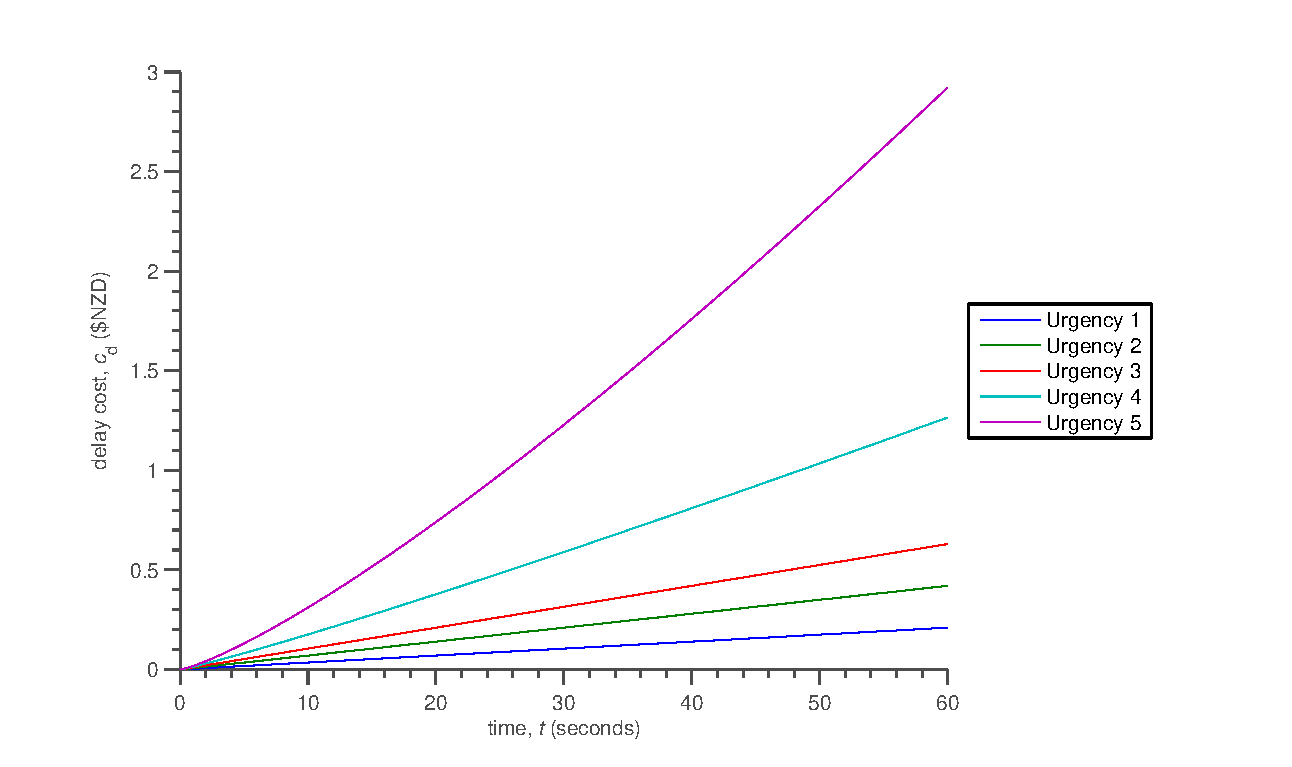
\includegraphics[scale=0.65]{delay_cost_per_urgency.eps}
	\caption{Cost of delay per time for a range of occupant urgency values, from time of zero seconds up to sixty seconds. }
\label{delaycosturgency}
\end{figure}

\section{PBTC System Design}
 
As no explicit information is available with respect to the costs of travel and delay for vehicles approaching a given intersection, modern traffic control algorithms typically attempt to reduce delay time or degree of intersection saturation in the hope of reducing congestion and improving the quality of travel. To reduce the costs of travel incurred by vehicles approaching a controlled intersection, the PBTC system is required to consider the costs of delay and stopping for approaching vehicles when making signal switching decisions. Vehicle-Controller communication is used to inform a PBTC traffic controller of the estimated costs using the models previously explained in this chapter, and the control algorithm is designed to allocate green time to phases based on aggregated cost estimates for approaching vehicles.

\subsection{Assumptions}

Design of a system for producing an optimal, minimal cost solution to phase assignment at any arbitrary controlled intersection is a difficult problem and evaluating such a system requires a sophisticated simulator capable of realistically modeling real world intersection geometrics, driver behaviours, and traffic flows. Development of these capabilities for simulation is an effort beyond the scope of this project. For this reason, the following assumptions have been made to simplify development of the PBTC control algorithm within this project:

\begin{itemize}
\item the control algorithm operates over a two-phase intersection, with each phase allocating green to one of two flows of traffic approaching the intersection only,
\item approaching vehicles represent straight through demand for the intersection only, no left/right split phases (i.e "arrow lights") are required,
\item the algorithm is limited to a single, isolated intersection only and does not consider any aspects of coordination between neighbouring intersection controllers.
\end{itemize}

\subsection{Vehicle-Controller Communication}

Communication between approaching or waiting vehicles and a PBTC controller at an intersection is required to provide inputs to the control algorithm to make a cost effective choice of phase timings based on the real-time traffic conditions. The implementation details of the required communication network is beyond the scope of this project and suggested as an area for future research. This project assumes that all of the necessary technology required for vehicles to send small packets of information to a controller exists in every vehicle using the road network, and each vehicle sends its own state information directly to the roadside intersection controller.

In the simulation developed as part of this project, vehicles approaching or waiting at a PBTC controlled intersection broadcast their current state to the intersection controller every two seconds if the distance to the intersection stop line is less than 150 metres. There are two justifications for this behaviour, firstly; although in a simulated environment any object can feasibly read the properties of any other object at any time, it is important to consider the real world application of the system where network latency and limited network capacity are real problems that prevent instantaneous, real-time messaging with no delay. 

Secondly, consider a situation where a single vehicle is approaching a red light at an intersection where there is no demand for the competing green phase; in a stop-line actuated control system the vehicle will be forced to stop, wait at least six seconds for the lights to react and change phase, and then take off. By allowing a 150 metre broadcast window, a PBTC controller is able to respond to this situation and change the phase before the approaching vehicle has reached the lights, preventing them from stopping. The 150 metre window is based on assuming an approaching vehicle is traveling at a constant speed below 80km/h (approximately 22 m/s), requiring at least 133 metres of clearance given a typical controller requires 6 seconds of inter-green time to change a phase. In practice, it might be useful to be able to tweak the distance at which cars would be considered by the PBTC system based on the speed limit of the area. 

\begin{figure}[]
\centering
	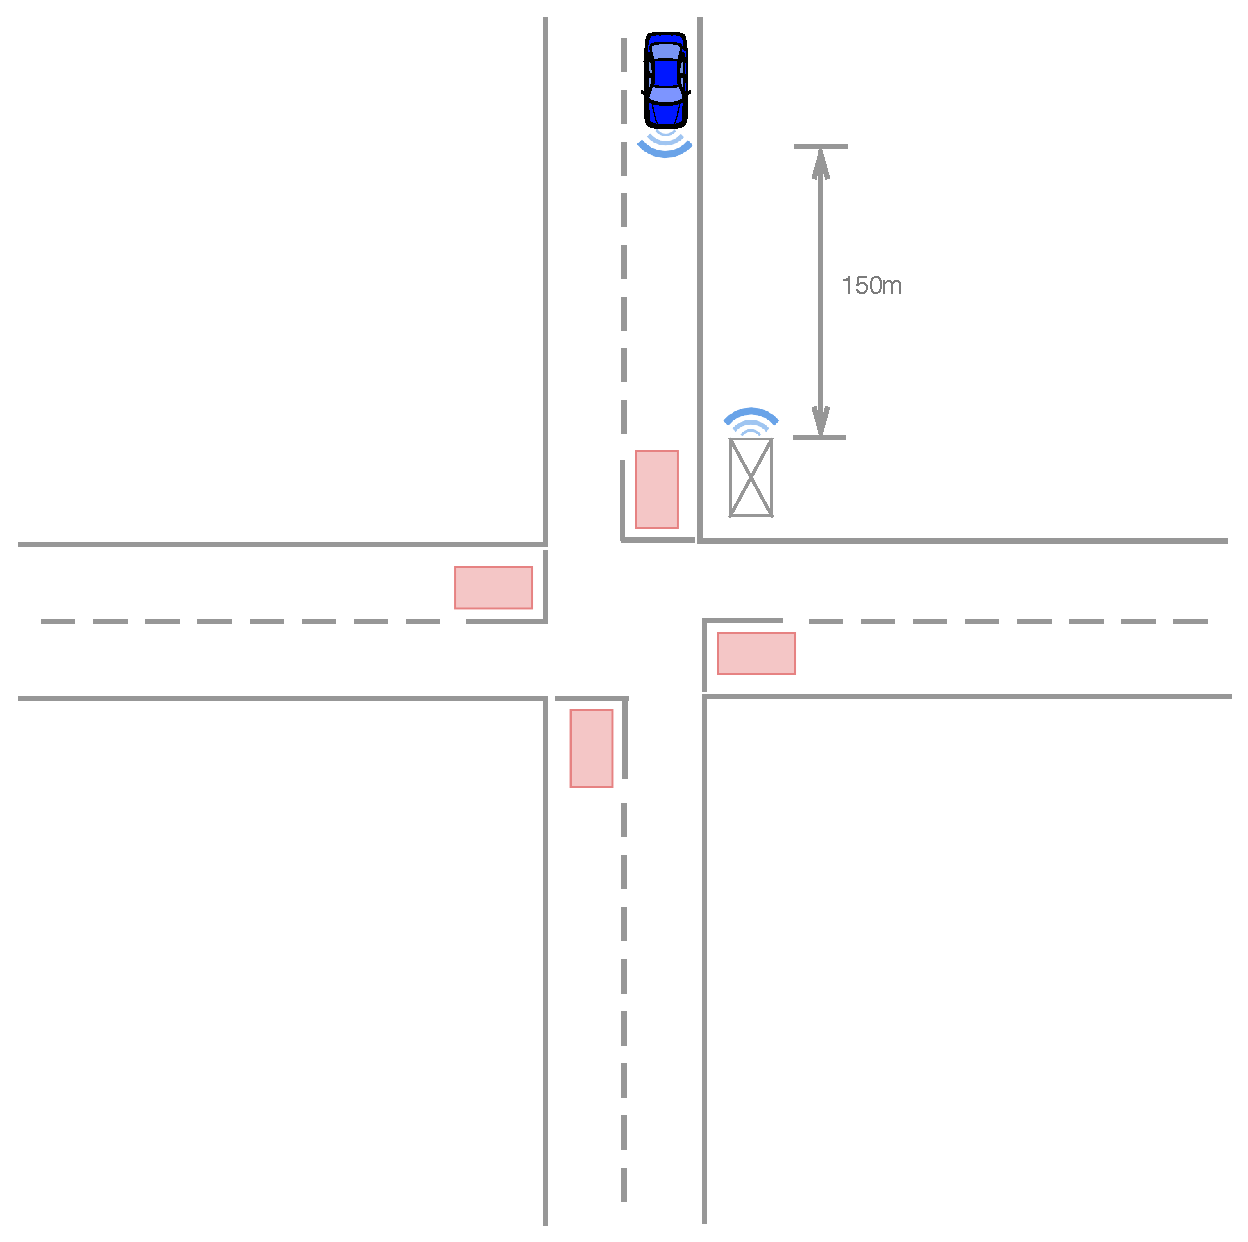
\includegraphics[scale=0.5]{intersection_diagram.eps}
	\caption{ Plan of a simple four way intersection showing an approaching vehicle communicating with a PBTC controller. The distance of initial communication is shown as 150 metres. The position of stop-line detectors typically used by SCATS systems are shown in red. The PBTC controller is able to adapt to vehicle actuations in advance of the vehicle's arrival at the stop line. }
\label{intersectiondiagram}
\end{figure}

\subsection {Control Algorithm Design}
\label{sec:PBTCDesign}

The PBTC control algorithm is a primary component of the PBTC system, designed to be executed by a roadside traffic controller to determine which phases should operate, the order of operation, and duration of each phase; in real-time. The primary objective of the PBTC control algorithm is to reduce the total economic cost incurred by vehicle movements  at PBTC controlled intersection, using traffic composition information communicated to a controller by vehicles in the network. The PBTC control algorithm is based on the delay time minimisation algorithm described by \citeasnoun{miller1963computer}, described in more detail in Chapter 2. The original algorithm presented by Miller has been extended to minimise delay and stopping cost rather than time spent delayed.

Phases of an intersection are preconfigured based upon the geometry of the intersection. Each phase within the PBTC system contains an allocation of green or red signals to each light at a controlled intersection, such that no two competing traffic flows receive a green light at the same time in a phase. Two traffic flows are said to be competing if a collision would occur if vehicles on each flow entered the intersection at the same time. Each phase also defines a minimum time the phase must run for.  The minimum time condition is a safety consideration of the system, designed to allow enough time for at least one vehicle to pass safely through the intersection before the phase is changed. 

The order and duration of phases at a PBTC controlled intersection is determined by calculating aggregate costs of delay and operation for each approach of an intersection. A PBTC controller maintains a list of messages received from approaching or delayed vehicles that are used for calculation of the delay costs and operational stopping costs for each vehicle and aggregated to find the total costs for an approach. The primary cost of changing phases at a controlled intersection is the cost of stopping and delaying free flowing traffic. As a result, the standard operation for a PBTC controlled intersection is to run a set phase continuously until a phase change is determined to be cost effective and scheduled by the PBTC control algorithm. This behaviour is designed to produce minimal changes to the system, effectively maximising the homogeneity of free flowing traffic until the cost of interfering becomes low relative to the cost of doing nothing. 

A phase change is scheduled by a PBTC controller if the sum of the cost of stopping the traffic flow currently approaching a green signal, defined as the phase change cost or $c_\text{pc}$, is less than the total incurred cost of delay for all vehicles queued and waiting at any approaches displaying a red signal, defined as the phase delay cost or $c_\text{pd}$. The cost of stopping the traffic flow on a green signal also includes an estimation of the potential delay cost for each vehicle assuming they must be delayed \emph{at least} as long as the minimum condition for the newly scheduled phase. Equations ~\ref{phaseChangeCostEq} and ~\ref{phaseDelayCostEq} define the phase change cost and phase delay cost. 

\begin{equation}
	c_\text{pc} &= \sum_{v \in A_\text{g}} c_\text{s}(v) + c_{\text{d}(min)}}(v)
	\label{phaseChangeCostEq}
\end{equation}

\begin{equation}
	c_\text{pd} &= \sum_{v \in A_\text{r}} c_\text{d}(v)
	\label{phaseDelayCostEq}
\end{equation}

Where $A_\text{g}$ denotes the set of vehicles approaching a green signal at the intersection, $A_\text{r}$ denotes the set of vehicles approaching or waiting at a red signal at the intersection, $c_\text{s}(v)$ is the incurred cost to a vehicle, $v$ if it is forced to stop, $c_{\text{d}(min)}(v)$ is the incurred cost of delay to vehicle $v$ for as many seconds as the minimum duration of the next phase, and $c_\text{d}(v)$ is the delay cost already incurred by $v$ due to waiting at a red signal.

If this condition is true at any time, the algorithm enters a phase change sequence. During a phase change sequence, a lookahead heuristic is applied to find the minimum potential cost incurred as a result of the change. Based on a predefined lookahead table size, the controller estimates the total cost of changing phase for each second from zero up to the table size, constructing a table with each row representing a time in seconds and the cost of stopping the phase at that time. The controller then dynamically extends the current phase duration by the number of seconds that corresponds with the lowest cost value in the lookahead table.

The lookahead method used in the PBTC control algorithm is an optimisation method performing a local search for a time of changing phases that incurs the least cost to the system. For example, consider an intersection where two vehicles have been waiting at a red signal for 60 seconds, and the cost of delay has exceeded the cost of stopping the opposing traffic flow receiving a green signal. If two vehicles are approaching the intersection on the freely flowing approach but are close enough to stop if the phase is changed immediately, the cost of the change includes the operational cost of stopping the two vehicles and the cost of delaying the vehicles for the minimum duration of the next phase. 

Due to their distance from the intersection and current velocity, after one additional second the two moving vehicles may pass through the intersection and these costs are avoided, with the trade-off cost being one more second of delay for the two waiting vehicles. Unless the two waiting vehicles have high urgency and a high number of passengers, the cost of an additional second of delay is likely to be marginal. The lookahead procedure of the PBTC control algorithm will evaluate the total cost of extending the current phase by a fixed number of seconds to allow the moving vehicles to pass, and extend the current phase by the calculated minimum time if it is found to be less than the cost of an immediate change.

\begin{algorithm}[H]
 \SetAlgoLined
 \KwData{
 	a: set of approaches, K: lookahead window size
 }
 \KwResult{ minimal cost time until phase should be change executed }
 \Begin{
  set $totalStoppingCost$ = 0 \; \\
  set $totalDelayCost$ = 0 \; \\
  \For{approach in approaches}{
  	\If{approach signal is red} {
		add cost of delay for all vehicles queued on approach to $totalDelayCost$ \;
	} 
	\Else{
		add cost of stopping and cost of minimum delay for all vehicles on approach to $totalStoppingCost$ \;
	}
  }
  \If {$stoppingCost < delayCost$} {
  	set lookaheadTable = [] \;
	\For{$i := 0$ to K} {
		lookaheadTable[i] = cost of delay for all stopped approaches over $i$ + cost of stopping for all vehicles that cannot clear the intersection after $i$ seconds \;
	}

  set extendedGreenTime = index of minimum value in lookaheadTable \;	
  return extendedGreenTime \;
}
return -1 \;	 \tcc*[r]{no change scheduled}
 }
 \caption{PBTC phase scheduling algorithm}
\end{algorithm}

% discuss lookahead search tree from other paper here

%The primary goal of the PBTC system is to reduce the economic costs of delay at a controlled intersection and as a result, evaluation metrics discussed here are designed to measure the impacted costs of running the system over an extended period of time for an intersection.








\chapter{Simulator Design and Implementation}

The following chapter describes the design and implementation of PBTSim, a software package to allow for simulation and evaluation of priority based traffic control. To produce a representative comparison with existing SCATS-based systems, creating a realistic simulation environment was a key implementation challenge, and a primary objective of this project. The outcomes discussed in this chapter are:

\begin{itemize}
\item using the open-source software package MovSim as a framework for implementation of PBTSim,
\item implementing a simulation scenario for development and evaluation,
\item extending the Movsim package within PBTSim to support development of the PBTC control algorithm and allowing for future control algorithms to be added easily,
\item development of a parser for SCATS log files, to allow for traffic flow rates and traffic signal phase timings to be read from a SCATS log file and used in simulation,
\end{itemize}

\section{Simulation Platform}

A primary challenge of measuring and evaluating performance of an adaptive traffic control system is the requirement to simulate realistic traffic conditions with sufficiently measurable results. Software for simulating traffic control methods is typically developed by vendors of a particular system and as such is proprietary and not available for research. Because of this, an open-source tool called Movsim has been used as a framework for development and evaluation within this project. 

Movsim (Multi-model Open-source Vehicular-traffic Simulator) is an open-source, Java-based traffic simulator implementing multiple time-continuous, car-following traffic models designed for investigating traffic dynamics; currently under active development. Movsim is based upon the work of \citeasnoun{kesting2013traffic} and implements a wide range of configurable vehicle-following, acceleration, and lane changing models that determine individual vehicle movement within the simulation.

\begin{figure}[]
\centering
	\includegraphics[scale=0.35]{movsim-interface.png}
	\caption{ A screenshot of the MovSim Graphical User Interface running a simulation of the four-way intersection scenario used during design and evaluation of the PBTC control system. }
\label{intersectiondiagram}
\end{figure}

All software artefacts produced during this project were implemented within a fork of the Movsim project, which we have named PBTSim (Priority Based Traffic Simulator). PBTSim is a software application that allows for simulation and evaluation of traffic control methods based on the vehicle priority model described in Chapter 4. While priority based traffic model features specific to this project are maintained in PBTSim, general purpose features and improvements to the Movsim project have been offered back to the original Movsim repository for consideration of the maintaining authors.

Limitations of using the MovSim project as a base simulation tool for the PBTSim include lack of support for bi-directional traffic flow and turning behaviour at intersections, both requirements for accurate modeling of a real world road network. Both of these features are areas of future development for the MovSim project. The sophisticated traffic modeling capabilities of the MovSim application, have outweighed these limitations during development of the PBTC system.

\section{Phase Model}

Movsim allows for customisable phases to be configured in the project description file, an XML document describing user-defined settings for traffic composition, simulation variables, and traffic controller plans. Traffic controller phases can be defined in the project description file as an ordered list, with each phase including a list of the state (green, amber, or red) for each traffic light for a given controller. 

\begin{figure}[]
\centering
	\includegraphics[scale=0.60]{movsim-phases.pdf}
	\caption{ A diagram of the available phase states and transitions of a "two-phase" configuration within the Movsim simulator. Movsim requires intergreen and all-red periods to be configured as individual phases and does not allow a simple mechanism for skipping, repeating, or alternating the order of configured phases. }
\label{movsimphasediagram}
\end{figure}

The phase model used in most modern traffic control systems is a finite state machine consisting of a set of states for each traffic light connected to the controller, with a set of constraints that define valid states and allowed transitions between states. The basic phase model implemented within the Movsim project implements this model, however Movsim requires a distinct phase for each period of intergreen time. For example, Figure ~\ref{movsimphasediagram} shows how a traditional "two phase" intersection requires a minimum of six configured phases to incorporate intergreen and all-red periods of operation using the Movsim model. This model requires more design and configuration effort, and does not enforce intergreen periods of operation between two active phases.

To solve this problem, a new phase model was developed for the PBTSim simulator during this project. The developed model is similar to the phase model used by SCATS, where each phase includes a fixed number of seconds as minimum time, maximum time, and intergreen time. It is assumed that during an intergreen period any traffic lights currently displaying a green signal transition to yellow, and all others remain the same. Using this model, the need for additional phases to explicitly define intergreen periods of operation is redundant and the PBTSim simulator enforces intergreen constraints between active phases. Figure ~\ref{PBTSimphasediagram} shows a state diagram of the PBTSim representation of the same "two phase" configuration described in Figure ~\ref{movsimphasediagram}.

\begin{figure}[]
\centering
	\includegraphics[scale=0.60]{pbtsim-phases.pdf}
	\caption{ A diagram of the available phase states and transitions of a "two-phase" configuration within the PBTSim simulator. Integreen and all-red times are encoded as properties of each phase and the scheduling of these phases is moved to application logic to simplify the phase configuration. }
\label{movsimphasediagram}
\end{figure}

%2
While appropriate for simple examples and fixed-time phases, the basic Movsim implementation of phase configuration is not appropriate for advanced controller strategies, including the PBTC strategy, where skipping phases with no traffic demand is desirable. It is difficult to express skipping of phases in the Movsim phase model, as there is no clear distinction between an intergreen phase and an "active" phase to indicate which phases are allowed to be skipped. For example, skipping the "next" phase will cause the traffic controller to skip the intergreen phase and change to another active phase, rather than the desired behaviour of skipping the next active phase.

The new phase model of PBTSim addresses this problem as integreen and all-red periods of operation are enforced during transitions between active phases, rather than phases themselves. As a result, expressing skipped phases or operating phases out of order is greatly simplified. 

The new phase model developed during this project has been provided to the Movsim authors as a potential general purpose improvement.

% good up to here jm 04.10.13

\section{Vehicle Priority Simulation}

Priority based traffic modeling is a concept specific to this project and is not implemented in any form within the Movsim simulator. To allow for implementation of the PBTC control system, PBTSim implements the priority model described in Chapter 4 for all vehicles, and simulates communication between vehicles and a traffic light controller as required by the PBTC control system.

\subsection{Traffic Composition}

The priority model described in Chapter 4 assumes that occupants of all vehicles on a road network have an urgency of travel, defined as a discrete integer between one and five. As this is an arbitrary, relative scale of motorist urgency, statistics of the distribution of driver urgencies for a given time or particular intersection are unknown and not easily measured.

As a result, the distribution of urgency values of traffic within the PBTSim system is estimated using an enumerated probability distribution which assigns an arbitrary probability of occurrence to each urgency value for each class of vehicle within the simulation. Table ~\ref{urgencydistribution} shows the probability distribution of urgency values for each class of vehicle in the PBTSim system. The distributions of urgency values are relatively weighted to indicate reasonable assumptions on vehicle urgency, which are difficult to empirically measure and it is beyond the scope of this project to do so, e.g. by surveying characteristics of vehicles and road users at an intersection. 

\begin{table}[]
\begin{center}
\begin{tabular}{lrrrrr}
\toprule
 & \multicolumn{5}{c}{Passenger Urgency} \\
 \cmidrule(lr){2-6}
Vehicle Class & 1 & 2 & 3 & 4 & 5 \\
\midrule
Car (Light Vehicle) & 0.2 & 0.25 & 0.395 & 0.15 & 0.005  \\
Bus (Heavy Vehicle) & 0.3 & 0.5 & 0.2 & 0.0 & 0.0 \\
Truck (Heavy Vehicle) & 0.1 & 0.5 & 0.3 & 0.1 & 0.0 \\
\bottomrule
\end{tabular}
\end{center}
\caption{Probability values for an enumerated integer distribution of individual vehicle urgencies. Each urgency value in the range 1--5 is associated with a probability of occurrence for a single vehicle. }
	\label{urgencydistribution}
\end{table}

Probability values are assigned to give a one-sided distribution that assumes there are lower proportions of truly urgent road users than not. Buses and trucks have relatively lower average urgency values compared to passenger cars. This measure is used to reflect that public transport is by its nature unreliable for each single passenger, hence most passengers using public transport allow more time than required to reach their destination and that the majority of freight trucks operate on long inter-city journeys, hence the proportion of time potentially spent waiting in traffic lights in a city is small compared to the relatively long journey time.

\subsection{Approach Communication}

A requirement of the design of the PBTC control system is that all vehicles approaching an intersection must broadcast their position, physical properties, and required passenger characteristics to a traffic controller. As Movsim was not designed with this requirement in mind, a new system of simulated communication between vehicles and traffic controllers had to be designed for the PBTSim simulator.

Each traffic controller within the simulation maintains a list of broadcasts they have received as a map and each new broadcast replaces any existing broadcast from each unique vehicle. An individual broadcast contains properties required by a controller in order to calculate operational stopping cost and delay cost estimated for each individual vehicle, specifically vehicle weight, speed, acceleration, urgency, number of passengers, and distance to the intersection stop-line. Once a vehicle has cleared the stop-line of an intersection, their broadcast is removed from the traffic controller map.

In order to ensure that the PBTSim environment is representative of a realistic road network and network infrastructure, efforts are made to ensure that the simulated communication between approaching vehicles and a traffic controller includes consideration of the challenges of a real-world communications network. In a simulated environment, vehicle properties can be broadcast instantly, without network costs or delay; however, in reality network topology and bandwidth limitations are factors that reduce the availability of broadcasts. To introduce consideration of networking latency into PBTSim, a two-second delay is imposed on each broadcast from an individual vehicle. This is not designed to be an accurate representation of network imperfections, but does reflect consideration of these factors.

An alternative design considered involved allowing delay and stopping costs to be calculated and broadcast by the vehicle itself. This method has the advantage of reducing the amount of calculations that are required to be made by a traffic controller, however this distributed computation is more difficult to implement successfully and there are no guarantees that all vehicles will implement the same cost calculations. This method is also difficult to update if changes to the cost calculations were desired after installation.

\section{Control Strategies}

Movsim includes a basic implementation of traffic control capable of operating an ordered list of traffic light phases defined in the simulation configuration file, however the implementation is limited to fixed-time phase control only, where each phase runs for a predetermined number of seconds before transitioning to the next phase. In order to allow for evaluation of multiple phase control strategies to be tested during simulation, a more sophisticated architecture design was implemented during development of the PBTSim system. 

Changes made to the traffic control architecture of PBTSim during this project are designed to be modular and avoid limiting the scope of future work or potential for implementation changes. Figure ~\ref{controllerclassdiagram} shows a UML class diagram of the type relationships in the traffic control architecture of PBTSim. ControlStrategy is a Java interface class added to PBTSim which implements the Strategy Pattern, an object-oriented design pattern that allows for dynamic selection of a strategy implementation at runtime. This pattern is well-suited to the design of the control strategy algorithm as new strategies (such as the PBTC system) can be added to the system by implementing the strategy interface and defining their own behaviour. % cite strategy pattern here

The ControlStrategy interface is called by a TrafficLightControlGroup class, which controls the state of lights within the simulator. Methods of the ControlStrategy interface allow a TrafficLightControlGroup to check if conditions for scheduling a phase change have been met and acknowledge the change once it has been made. Each concrete implementation of the ControlStrategy class can implement their own conditions and strategies that will trigger a change. This relationship creates a separation of concerns between controlling traffic light state and defining traffic light behaviour, allowing for new behaviours to be easily added independently of all other existing strategies. 

\begin{figure}[]
\centering
	\includegraphics[scale=0.60]{controller_class_diagram.pdf}
	\caption{ A UML class diagram showing the use of the strategy pattern between the TrafficLightControlGroup and ControlStrategy types. ControlStrategy is an interface defining methods required by the TrafficLightControlGroup to change the phase of a set of traffic lights. Three strategies implementing the ControlStrategy interface are shown. Each concrete strategy implementation has a different internal set of conditions to trigger phase changes. }
\label{controllerclassdiagram}
\end{figure}

% good up to here

\section{Implementation of the PBTC Control Strategy}

The PBTC control algorithm described in Section ~\ref{sec:PBTCDesign} is implemented as a concrete ControlStrategy implementation within PBTSim. The strategy implementation of the PBTC control algorithm consists of two primary phases of operation; approach cost calculation and phase scheduling. 

The PBTC control algorithm implementation dynamically calculates the sum of the individual estimated delay and operational stopping costs for all of the vehicles on each approaching link of the intersection at each simulator update. 
The current phase of a PBTC traffic controller operates continuously until the calculated cost of delay on all stopped approaches exceeds than the cost of stopping green approaches, at which point the next phase is allocated and the controller enters the phase change sequence. Once the controller has entered the phase change sequence, it is  committed to changing phases and the lookahead optimisation method is employed to determine whether the phase should change now, or some point in the future, based on the real-time position and state information of vehicles on approaching links. 

% this section is good
\subsection{Lookahead Optimisation}

PBTSim implements the PBTC control algorithm's lookahead features using a map to construct a table of cost values a the end of each phase, once the phase change sequence has been initiated. The lookahead table includes an estimate of the instantaneous change costs for all vehicles known to the PBTC controller at the time the phase change sequence was entered. For each second up to the defined size of the lookahead table, $K$, the PBTC control strategy estimates the cost of changing phases by finding the sum of the cost of stopping, and the cost of delay at least equal to the minimum duration of the next phase in the controller sequence for every individual vehicle approaching a green signal, and the sum of the cost of stopping and cost of delay for the duration of the current lookahead for any vehicles approaching or queued at a red signal. 

To estimate the costs of a phase change each second up to the lookahead time, a PBTC system needs to identify if each vehicle approaching a light currently displaying a green signal will be stopped by the phase change and hence incur the cost of stopping, or will clear the intersection within the number of seconds the change will be scheduled for and have no additional costs incurred. In a free-flowing traffic situation, the distance traveled by a vehicle in a fixed time frame can be estimated using the vehicles speed and acceleration only. For example, if a PBTC controller is considering a phase change for an intersection 5 seconds from the present time, and a vehicle is approaching at 10m/s at a distance of 30 metres, the vehicle will have passed over the intersection stop line within 3 seconds therefore will not be affected by the phase change.  However, in congested traffic where vehicles are queued, whether or not a given vehicle, $v$ in the queue will clear an intersection within $t$ seconds is dependant on the speed and acceleration profiles of vehicles in front of $v$, and as a result is significantly affected by driver behaviours and instantaneous traffic conditions. 

Developing and implementing such a model for simulation and evaluation of the PBTC system is an effort beyond the scope of this project and as a result, empirical measurement of clearance times and distances within PBTSim was conducted to estimate the worst-case conditions of congested traffic and identify the maximum distance a vehicle could be from a traffic light to clear within a fixed range of seconds. The experiment was run by operating a green phase for a fixed number of seconds at an intersection with a volume of traffic exceeding the capacity of the network, to generate a queue. The distance of the furtherest vehicle from the intersection at the time that the phase began that cleared the intersection within the time frame is the result, repeated a number of times to find a maximum. 

Measurement results were used to create a map of key-value pairs consisting of the time in seconds, and the maximum distance from a traffic light a vehicle could expect to clear the intersection within the time frame. Table ~\ref{vehiclecleardistances} shows the measured results used by PBTSim to determine whether each vehicle will clear a traffic light within a given timeframe. If a vehicle has a speed of less than 2.5m/s when approaching a traffic light, it is assumed to be in queue and the estimated clear time is determined from the table.

\begin{table}[]
\begin{center}
\begin{tabular}{rr}
\toprule
Phase Duration ($s$) & Queue Clear Distance ($m$) \\
\midrule
10 & 22.12 \\
15 & 40.03 \\
20 & 58.10 \\
25 & 80.15 \\
30 & 94.40 \\
35 & 111.47 \\
40 & 133.50 \\
\bottomrule
\end{tabular}
\end{center}
\caption{ Estimated maximum intersection clearance distances used by PBTSim to determine if a queued vehicle will pass an intersection before the end of a phase. The time is given as the duration of green time remaining in the phase, and the distance is the maximum expected distance a vehicle can be queued from the intersection stop-line to clear within the allowed time. }
\label{vehiclecleardistances}
\end{table}

\section{Implementation of a SCATS Control Strategy}

% can use the SCATS data to determine arrivals and signal settings each cyclex
Development of a SCATS representation is a requirement of the evaluation process of this project. As SCATS is deployed on most of the controlled intersections within New Zealand and uses an adaptive traffic control algorithm to respond to near real-time traffic demand, it is appropriate for comparison with the PBTC control algorithm.

As SCATS is a commercial system, no software or algorithms are available for public research. As a result, the SCATS implementation developed for PBTSim is designed to recreate a realistic representation of real-world SCATS behaviour using an available log file of vehicle arrivals and allocated phase times at different intersections in Wellington City. An example of the SCATS log file format is shown in Appendix A. Log files for intersections in Wellington City were provided for a 12 hour period of a typical day by the Wellington City Council.

Each SCATS log file consists of an ordered sequence of data blocks for each single cycle of operation of a given traffic light controller, sent to SCATS by the controller at the end of each cycle. The cycle block contains state information required by SCATS to calculate the phase timings for the next cycle, including number of vehicle detector actuations per approach, i.e. the number of vehicles that entered the intersection on each approach; and the order and time of each of the phase splits run by the controller during that cycle. 

The design and implementation of a software package to simulate SCATS behaviour involved replicating the arrivals recorded by SCATS over the fixed period of the log, and developing a control strategy to operate phase times for each cycle of the log. Figure ~\ref{scatsclassdiagram} shows a class diagram overview of classes in PBTSim designed to add SCATS simulation capabilities. 

% good up to here
\subsection{Vehicle Arrivals}

The number of vehicles arriving or waiting at an intersection, also referred to as the saturation or flow rate of an intersection, is an independent variable determined by the number of vehicles on the road, criticality of an intersection to a road network. When comparing the performance of multiple traffic control strategies, the flow of vehicles input into the system should remain constant between each experiment. To account for this in the evaluation of the PBTC control system, SCATS log files are used to determine the flow rate of vehicle arrivals in PBTSim. 

SCATS provides the number of vehicle actuations recorded by each stop line inductive loop detector, for each cycle contained within an intersection log file. As SCATS detectors are placed on the stop line of each approach at an intersection, it is assumed that the number of vehicle actuations at each detector is approximately equal to the number of vehicles that passed through the intersection during a given green phase and the number of vehicles that arrived on that approach over the entire cycle. By using the cycle duration as a range for estimating the exact arrival time of a given vehicle approaching an intersection, it is possible to introduce a probability function that allows for a proportion of vehicles to arrive early during a red phase, and the remainder to arrive on time during the green phase of a particular traffic light. As no other information related to the time of vehicle arrivals is available, arrival events are implemented using a Poisson arrival process. 

During a PBTSim simulation, the Poisson process is used to generate an estimated time to the next arrival after each simulated arrival has taken place. The Poisson arrivals implementation is a general purpose improvement over the linear arrivals model that was previously implemented in Movsim has been submitted back to the original Movsim repository as a configurable option to benefit other research.

These assumptions provide a reasonable estimate of the arrival time of vehicles to each queue at an intersection, as it is not possible to know the exact time of arrival and waiting time for each vehicle using only SCATS log files. The consequence of these assumptions is that generated arrival times may not be representative of the arrival times that occurred during the real-world scenario that the SCATS log files reflect, although on average it is expected the simulated arrival times will be close approximations of real-world arrivals. 

\subsection{SCATS Control Stategy}

The SCATS representation developed for PBTSim is designed to implement the ControlStategy interface class to work seamlessly with the traffic lights and controller classes of PBTSim.

The SCATSDataControlStrategy is a Java class that dynamically operates the measured phase durations contained within a SCATS log file by requesting new data from the SCATSDataParser each cycle. The SCATSDataParser is a singleton class which waits for a prompt for data from a SCATSDataControlStrategy or TrafficSource instance. The parser reads a cycle block from the log file and returns a list of phases and their durations to the SCATSDataControlStrategy, and updates each TrafficSource with a new arrival flow rate based on the phase times and vehicle arrivals measured in current cycle being read from the SCATS log. The SCATSDataControlStrategy allocates phases in order based on the list returned from the data parser and continues until the list is empty, at which point it requests another cycle and so forth.

The SCATSDataParser class is designed to respond to requests for data as it does not implement its own update method so does not have a measure of simulation time elapsed. This method ensures that a new cycle is only read from the log after the previous cycle has ended. One disadvantage of this method is that individual timers kept by each TrafficSource are not synchronised so after the cycle duration has expired, each individual TrafficSource will attempt to request the data parser to read a new cycle. Multiple cycle reads are avoided by reseting each TrafficSource after the first one has called for an update.
























\chapter{Evaluation}
\label{chapter:evaluation}

\section{Methodology}

Performance evaluation and analysis is required to determine the effectiveness and appropriateness of the PBTC system. Performance evaluation of traffic control methodology is made difficult by the proprietary and commercial nature of traffic control algorithms and the software systems that implement them. In New Zealand, intersections are controlled by the SCATS system, which is commercially developed in Australia and in use in many countries worldwide. No test bed or performance evaluation software is available for SCATS, and as a result a direct comparison with the SCATS implementation is not possible.

An alternative to a direct comparison with the SCATS system considered during the development of this project was to develop a simplified and approximate system that was based off the methodology of SCATS. While this method has the advantage of being able to produce a flexible estimation system that can be easily benchmarked against the PBTC system, there are disadvantages related to implementing an approximation to be representative of the real system. Firstly, there is a limited amount of publicly accessible information related to the design and implementation of the SCATS control algorithms. One of the very few papers available described some algorithms of the very first version of the SCATS system \citeasnoun{lowrie1982scats}, however it is not easy to know how much the system has improved since this paper was published. Secondly, it is not easy to determine how good of an approximation any simplified implementation of SCATS would be without being able to benchmark against the real system leading to potentially inaccurate comparisons. 

As a result of these two limitations, the evaluation component of this project was designed based on using reports generated by SCATS containing phase times and traffic conditions of the SCATS system operating on intersections in Wellington over a 12 hour period. The reports used during evaluation were provided by the Wellington City Council (WCC), who operate SCATS for all of the intersections in the central Wellington City area. SCATS allows WCC engineers to produce report logs showing data and intersection state information for every cycle of operation, including exact phase times and the number of vehicle detections per phase. The evaluation component of this project was designed to use the information contained within these reports to reconstruct a realistic representation of SCATS operation in Wellington. This method was preferred over the custom implementation of SCATS because of the relative ease of generating vehicle arrivals and scheduling phase times based off the SCATS reports in simulation.

Traffic demand on road networks is typically time varying, and the flow of traffic in urban centres typically peaks in the early morning and early evening periods, corresponding with commuters travelling to and from workplaces within the city, to urban or suburban residences. The 13-hour period of operation was determined with consideration to the typical profile of traffic in the central Wellington City area during a day, characterised by two "peaks" of high volume in the morning and evening for around 1-2 hours each. By evaluating traffic performance over a 13-hour period from 6:00 a.m. to 7:00 p.m., these peaks can be included in the evaluation, creating a range of traffic conditions for performance analysis. 

\section{Experimental Configuration}

Evaluation of the PBTC control strategy, Vehicle Actuated control strategy, and SCATS representation was carried out within the developed PBTSim application to measure and analyse the impact of control strategy heuristics with regards to incurred delays and costs imposed on vehicles within a simulation. The experimental configuration consisted of three simulated intersection configurations, based on real-world intersections within central Wellington City; namely the intersections of Vivian Street and Victoria Street, Victoria Street and Karo Drive, and Courtney Place and Tory Street. Appendix ~\ref{scats_i

% describe the traffic configuration settings
Traffic volume was simulated by parsing vehicle detections from SCATS log file for each of the three evaluation intersections. SCATS provided by the WCC contained 13 hours of data logged on the 20th June, 2013. A static traffic composition configuration of 80\%-20\% light vehicles - heavy vehicles was used for all of the simulation runs during evaluation.

Each simulation run was repeated ten times for each of the tree controller strategies evaluated by this project, on each of the three evaluation intersections, for a total of 90 unique runs. Post-processing tools were used to report the mean and standard deviation of results for each set of repeated runs. Metrics were analysed post-experimentation using MATLAB. The set of results generated by each simulation run include the following evaluation metrics:

\begin{itemize}
\item Mean number of vehicle arrivals over each 30 second window of simulation
\item Mean delay time, cost of delay, and incurred costs of stopping for each vehicle during simulation
\item Delay time, cost of delay, and incurred costs of stopping of all vehicles over each 30 second window of simulation
\item Total delay time, cost of delay, and incurred costs of stopping for all vehicles during simulation
\end{itemize}

The Vehicle Actuated traffic control strategy was set to a fixed phase duration of 30 seconds, with minimum and maximum duration limits of 15 and 60 seconds, respectively. Simulated detectors for the Vehicle Actuated strategy were placed 5 metres from the stop line. The geometric layout of each PBTSim intersection configuration was constructed to reflect the real-world geometry of each intersection, with lanes not used in the evaluation omitted. 

\section{Traffic Flow}
\label{sec:trafficflow}

To investigate the flow of traffic through the simulation networks over the course of the simulation period, the number of vehicle arrivals was logged every 30 seconds of simulation time. The flow of traffic over a 13 hour period during a typical day can be expected to vary, and the performance of different traffic management strategies may be affected by periodic flow rates. Traffic flow within the experimentation was generated from detector data contained within the SCATS log files of each intersection. Figure ~\ref{eval:vehiclearrivalstime} shows a plot of the trend in vehicle arrivals over the simulation period for each of the evaluation intersections. Each of the three intersections show evidence of ``peak'' traffic periods, typically during the first 3 hours and last 3 hours of the evaluation window.

The Vivian-Victoria intersection has significantly higher traffic flow than the other two intersections evaluated. As the inbound link of the southern motorway, Vivian Street is an arterial link of Wellington's road network and a typical route for many Hutt Valley commuters working in the central business district (CBD). This is evidenced in ~\ref{vehiclearrivalstime:sub1}, flow recorded on the Vivian Street approach is considerably higher than Victoria Street for the majority of the evaluation window. The flow recorded at the Courtenay-Tory intersection is relatively low. As neither Courtenay Place or Tory Street are motorway approaches, the comparably lower rate of traffic flow is expected. 

The Karo-Victoria intersection shows clear evidence of morning and evening traffic peaks, with flow increasing up to the end of the evaluation period, which corresponds approximately 7pm in real-time. As Karo Drive is the entry to the northern motorway, and one of the few routes by which Hutt Valley commuters can easily leave the CBD, the end-of-day flow increase is expected. The flow rate at the Victoria Street approach to the Karo intersection remains consistently low over the entire evaluation period. From personal experience of traveling via this intersection, more than one vehicle per 30 seconds is expected on this approach which suggests the SCATS log file may be incomplete (for example, due to a failed detector) and is not reflecting the real traffic flow at that intersection. 

\begin{figure}
\centering
\begin{subfigure}{.5\textwidth}
  \centering
  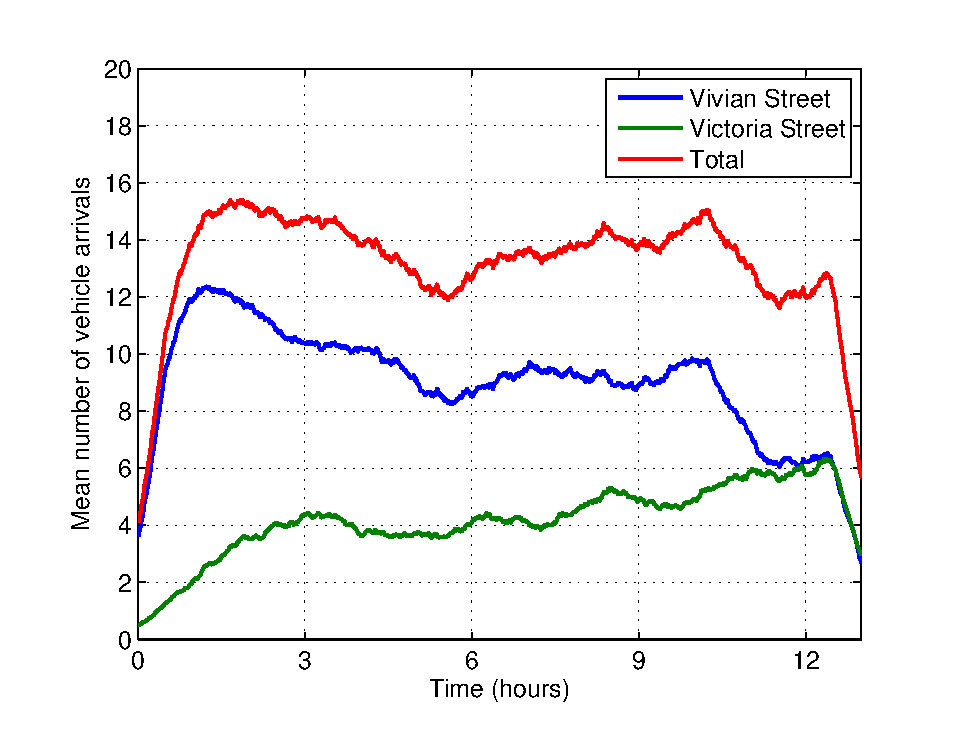
\includegraphics[scale=0.50]{vivian_victoria_num_arrivals_time.eps}
  \caption{A subfigure}
  \label{vehiclearrivalstime:sub1}
\end{subfigure}%
\begin{subfigure}{.5\textwidth}
  \centering
  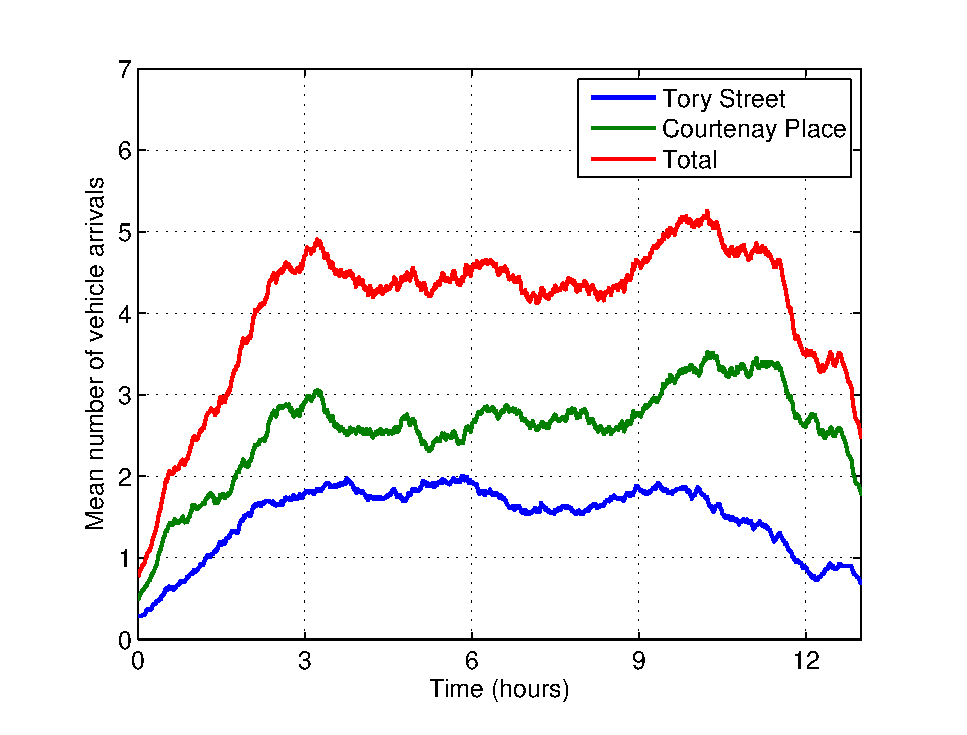
\includegraphics[scale=0.50]{courtenay_tory_num_arrivals_time.eps}
  \caption{A subfigure}
  \label{vehiclearrivalstime:sub2}
\end{subfigure}

\vspace{1cm}

\begin{subfigure}{.5\textwidth}
  \centering
  \includegraphics[scale=0.50]{karo_victoria_num_arrivals_time.eps}
  \caption{A subfigure}
  \label{vehiclearrivalstime:sub3}
\end{subfigure}%
\caption{ A plot of the trend in the mean number of vehicle arrivals per 30 seconds over the duration of the evaluation window of 13 hours for each of the evaluation intersections. The mean number of vehicle arrivals for each 30 second block is determined through use of a convolution filter to display a moving average per hour of simulation time. The filtered data effectively displays an overview of the trend of traffic flow at each hour of the evaluation window. The flow rate at all three intersections shows evidence of expected morning and evening peaks caused by worker commutes. }
\label{eval:vehiclearrivalstime}
\end{figure}

\section {Delay Time and Cost}
\label{sec:incurred_delay_cost}

Delay time and delay cost are related metrics, though the relationship is not directly proportional as the cost of delay for an individual vehicle is determined by a function of urgency as well as time. As the SCATS and Vehicle Actuated control strategies do not consider delay cost when making phase control decisions, the total time vehicles are delayed is a valuable metric for these two systems, and is a metric often raised in informal discussions related to the effectiveness of traffic lights, as the individual delay time is the most noticeable cost to road users at controlled intersections.

Figure ~\ref{eval:approaches_delay_time} shows a plot of the mean time spent delayed by individual vehicles within the experimental simulation, distributed by vehicle urgency for each of the three control strategies evaluated. The PBTC control system is able to achieve lower mean delay times across each of the three intersections, most appreciably on the intersection of Karo Drive and Victoria Street. The Vehicle Actuated control strategy typically results in the longest mean delay times, although performance is improved over the SCATS control strategy on the Karo-Victoria intersection. A possible reason for this performance is that the fixed phase duration of the Vehicle Actuated strategy is appropriate for the traffic flow at this intersection. The SCATS controller consistently results in longer mean delay times across all vehicle urgencies for the Courtenay-Tory and Karo-Victoria intersections when compared to PBTC, but it able to achieve lower mean delay times compared to PBTC on the intersection of results comparable to PBTC for the intersection of Vivian Street and Victoria Street. It is also possible that the reason for the degraded SCATS performance on the simulation of Karo-Victoria is due to an incomplete or non-representative log file, as described in \ref{sec:trafficflow}. 

The difference in mean delay time between the PBTC system and SCATS or Vehicle Actuated systems appears to be more pronounced on the Karo-Victoria and Courtenay-Tory intersections. One possible reason for this is the lower volume of traffic on each of these intersections, suggesting that the performance benefits of the PBTC system are higher in ligher traffic scenarios, as the PBTC controller can favour shorter phase durations to result in lower delay times. 

The PBTC control system also shows evidence of urgency preference within the mean delay times recorded per urgency. There is a decreasing trend in mean delay times recorded by the PBTC control system for increasing urgencies, which reflects that the PBTC control system considers cost of delay as a function of time and urgency when making control decisions. The SCATS and Vehicle Actuated control strategies do not show any evidence of this trend, as expected.
% note that there are significantly less priority 5 vehicles

\begin{figure}
\centering
\begin{subfigure}{.5\textwidth}
  \centering
  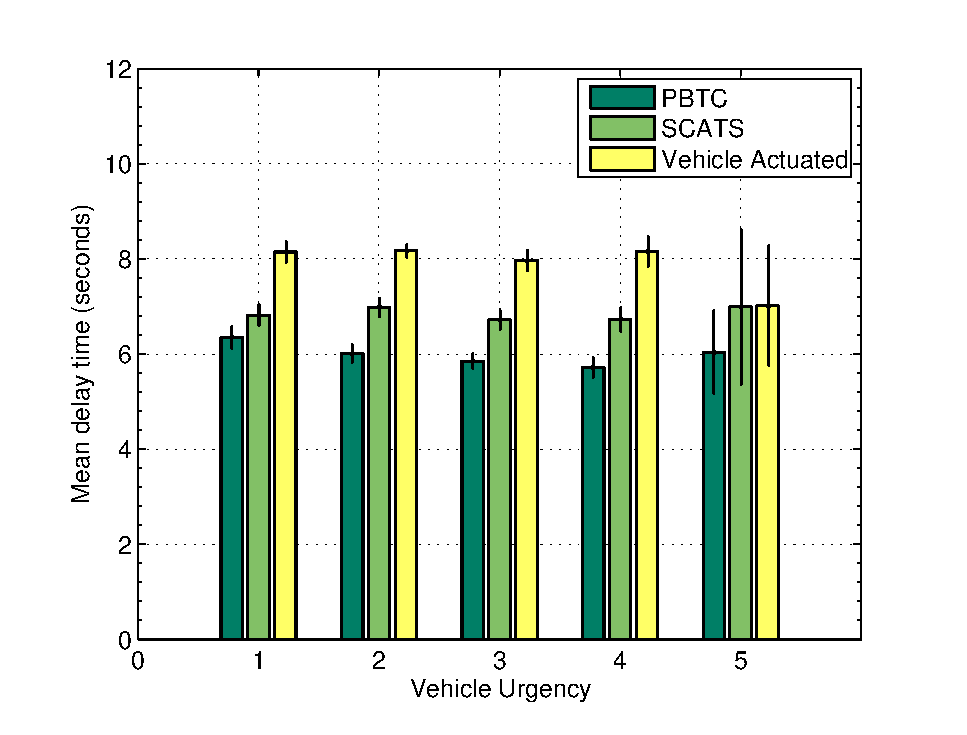
\includegraphics[scale=0.50]{vivian_victoria_approaches_delay_time.eps}
  \caption{Victoria-Vivian}
  \label{approaches_delay_time:sub1}
\end{subfigure}%
\begin{subfigure}{.5\textwidth}
  \centering
  \includegraphics[scale=0.50]{courtenay_tory_approaches_delay_time.eps}
  \caption{Courtenay-Tory}
  \label{approaches_delay_time:sub2}
\end{subfigure}

\vspace{1cm}

\begin{subfigure}{.5\textwidth}
  \centering
  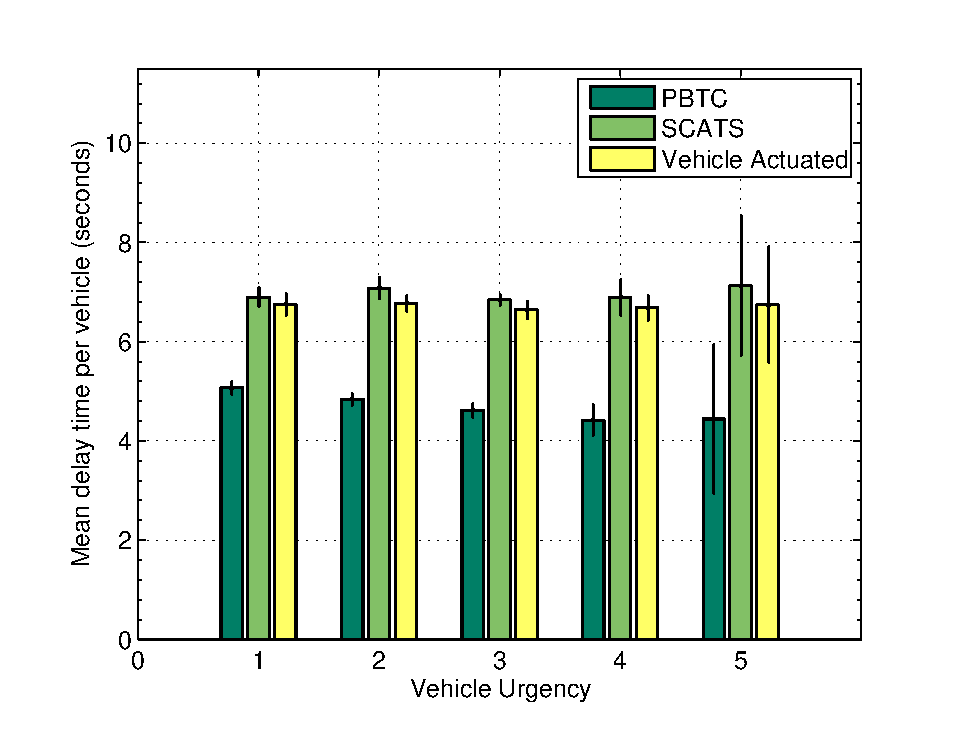
\includegraphics[scale=0.50]{karo_victoria_approaches_delay_time.eps}
  \caption{Karo-Victoria}
  \label{approaches_delay_time:sub3}
\end{subfigure}%
\caption{ A bar chart of the mean delay time, measured in seconds, for an individual vehicle in the experimental simulation for each of the three evaluation intersections. The PBTC control system outperforms SCATS and Vehicle Actuated controls over all of the dimensions.  }
\label{eval:approaches_delay_time}
\end{figure}

The PBTC system similarly outperforms the SCATS and Vehicle Actuated control strategies when considering the mean incurred cost of delay for individual vehicles within the experimental simulation. Figure ~\ref{eval:approaches_delay_cost} shows a bar chart of the delay cost, for each of the three control strategies and grouped by vehicle urgency. 

All three control strategies display a clear trend of increasing costs as vehicle urgency increases, expected as per the design of the delay cost measure, described in ~\ref{sec:design_delay_cost}. The PBTC control system consistently results in a lower mean delay cost for all vehicles in each simulation run. As with delay time, the Vehicle Actuated control strategy performs the worst with respect to delay cost over all three simulated intersections. From this result, we conclude that the fixed phase design of the vehicle actuated control strategy results in longer stoppages for traveling vehicles and as a result a higher delay cost. The SCATS and Vehicle Actuated control strategies both perform significantly worse with respect to the cost of high urgency (4-5) vehicles. Because the PBTC control system identifies and prioritises traffic based on urgency, the mean delay cost for higher urgency vehicles is relatively decreased.

 The standard deviation displayed on each of the charts is also more significant for urgency 5 vehicles. There are two possible reasons for this increased error; firstly, there are typically less than 5\% urgency 5 vehicles in each simulation as per the urgency distribution displayed in ~\ref{urgencydistribution} and as a result the probability of delay for an urgency 5 vehicle is higher. Futhermore, as the relationship between time and delay cost for urgency 5 is greater, smaller differences in the delay time develop into larger delay costs and more significant error over a small sample.
 
As with delay time performance, the chart ~\ref{approaches_delay_cost:sub3} shows the SCATS system consistently performs worse that both the PBTC and Vehicle Actuated strategies on the Karo Drive and Victoria Street intersection.

\begin{figure}
\centering
\begin{subfigure}{.5\textwidth}
  \centering
  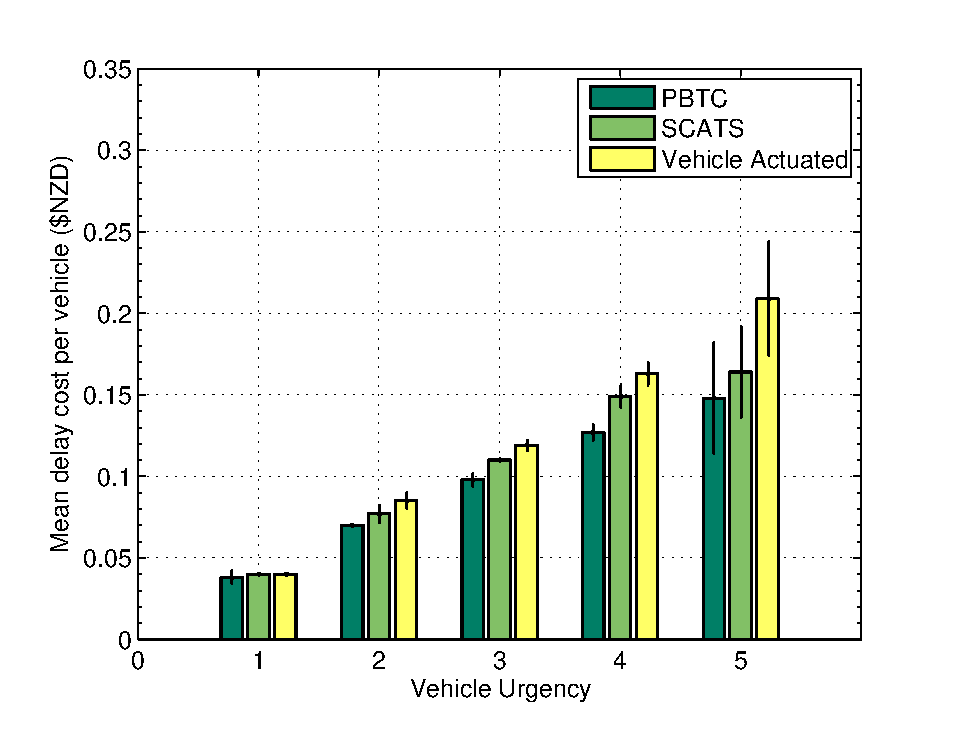
\includegraphics[scale=0.5]{vivian_victoria_approaches_delay_cost.eps}
  \caption{Vivian-Victoria}
  \label{approaches_delay_cost:sub1}
\end{subfigure}%
\begin{subfigure}{.5\textwidth}
  \centering
  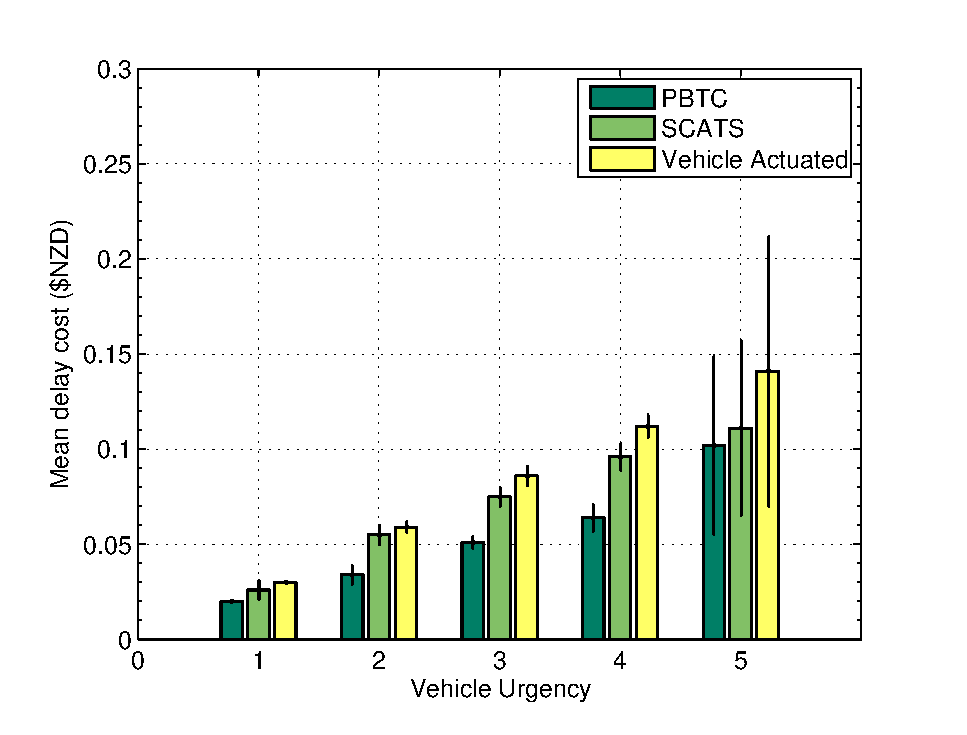
\includegraphics[scale=0.5]{courtenay_tory_approaches_delay_cost.eps}
  \caption{Courtenay-Tory}
  \label{approaches_delay_cost:sub2}
\end{subfigure}

\vspace{1cm}

\begin{subfigure}{.5\textwidth}
  \centering
  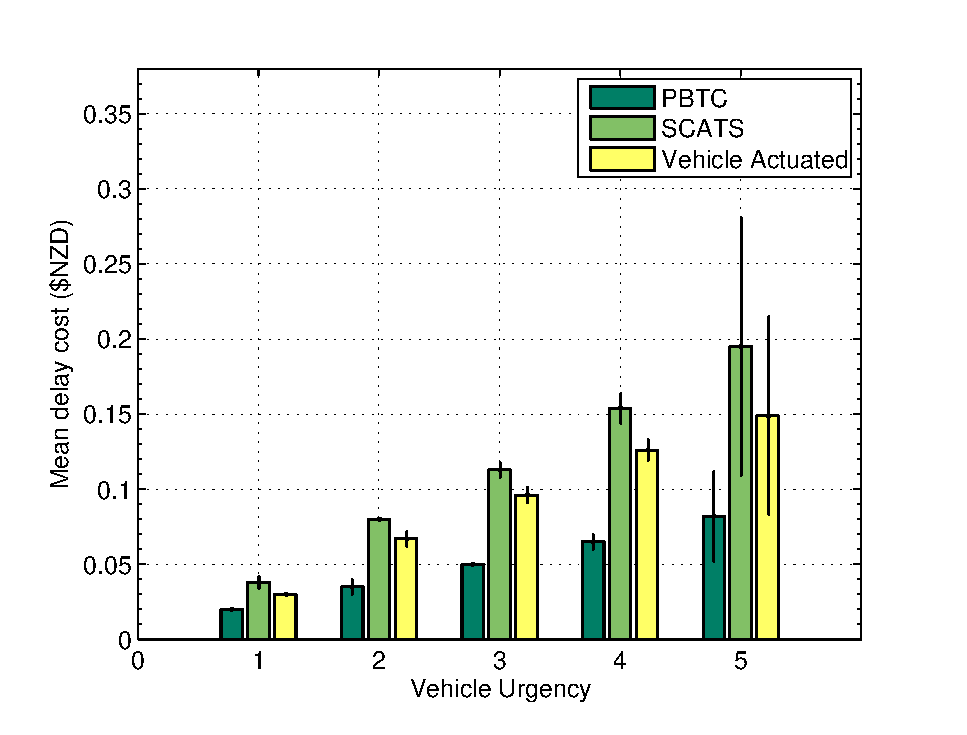
\includegraphics[scale=0.5]{karo_victoria_approaches_delay_cost.eps}
  \caption{Karo-Victoria}
  \label{approaches_delay_cost:sub3}
\end{subfigure}%
\caption{ A bar chart of the mean delay cost, in New Zealand Dollars, for an individual vehicle in the experimental simulation for each of the three evaluation intersections. The PBTC control system outperforms SCATS and Vehicle Actuated controls over all of the dimensions.  }
\label{eval:approaches_delay_cost}
\end{figure}

Further analysis of the incurred delay costs for vehicles over each of the control strategies can be made by considering the mean cost per hour of simulation time to evaluate the change in delay cost between the three systems on each intersection over the duration of the evaluation period.Figure  ~\ref{eval:delay_cost_time} shows a plot of the mean delay cost per hour of simulation time over each of the three evaluation intersections and control strategies. 

\begin{figure}[H]
\centering
\begin{subfigure}{.5\textwidth}
  \centering
  \includegraphics[scale=0.5]{vivian_victoria_delay_cost_time.eps}
  \caption{Vivian-Victoria}
  \label{delay_cost_time:sub1}
\end{subfigure}%
\begin{subfigure}{.5\textwidth}
  \centering
  \includegraphics[scale=0.5]{courtenay_tory_delay_cost_time.eps}
  \caption{Courtenay-Tory}
  \label{delay_cost_time:sub2}
\end{subfigure}

\vspace{1cm}

\begin{subfigure}{.5\textwidth}
  \centering
  \includegraphics[scale=0.5]{karo_victoria_delay_cost_time.eps}
  \caption{Karo-Victoria}
  \label{delay_cost_time:sub3}
\end{subfigure}%
\caption{ A plot of the mean delay cost per hour for each of the PBTC, SCATS, and Vehicle Actuated control strategies as applied to each of the three evaluation intersection configurations. Each plot line displays an indication of the trend in delay cost over the period of a day. The PBTC and SCATS strategies typically achieve lower costs between 3 and 9 hours of simulation time, which is clear evidence that these control strategies can adapt to the lower traffic volumes over this time period. The Vehicle Actuated control strategy does not adapt phase times and the mean delay cost recorded per hour is significantly higher and relatively consistent; with the exception of the Karo-Victoria intersection where the Vehicle Actuated strategy performs very well suggesting that the fixed phase times of this plan were a good fit for the traffic flow at this intersection over the evaluation period. }
\label{eval:delay_cost_time}
\end{figure}

The charts presented in Figure~\ref{eval:delay_cost_time} show a clear illustration of the difference between the adaptive PBTC and SCATS control strategies, and the non-adaptive Vehicle Actuated strategy. The mean delay cost for both the PBTC and SCATS control strategies tends to peak both in the AM period between 0 and 3 hours of simulation time and the evening period beyond 9 hours of simulation time, with a period of lower mean delay cost per hour in between. The adaptive effect is most prominently displayed on charts ~\ref{delay_cost_time:sub1} and ~\ref{delay_cost_time:sub2}, corresponding to the intersections of Victoria Street and Vivian Street and Courtenay Place and Tory Street, respectively. A greater understanding of the relationship between delay cost and traffic flow can be found by comparing these results to the trend in traffic volume over the same period, as shown in Figure ~\ref{eval:vehiclearrivalstime}. The observed relationship indicates lower delay costs can be achieved by the PBTC and SCATS strategies as traffic volume decreases during the middle of the day period. This is in contrast to the results of the Vehicle Actuated system, where the mean delay cost per hour is relatively consistent over the entire period of a day, evidence of the fixed, non-adaptive nature of the Vehicle Actuated strategy.

The trend in mean delay cost per hour between the PBTC and SCATS control strategies is observed to be similar over the period of evaluation at the Vivian Street and Victoria Street intersection, as shown in chart ~\ref{delay_cost_time:sub1} . The plot of delay cost and time for the two systems follow a similar pattern, however the PBTC system achieves consistently lower delay costs across this period. This result is evidence of the incremental adaptation algorithm used by the SCATS system to adjust phase duration. SCATS and PBTC both adjust their phase times to meet the volume of demand at an intersection, though SCATS is an incremental adjustment based on near real-time flow and the PBTC system is a direct adjustment based on vehicles present in real-time, hence adjustments made by the SCATS system are slower to take effect.

In contrast, SCATS is observed to perform relatively worse than both the PBTC and Vehicle Actuated control strategies over the peak traffic period at the intersection of Karo Drive and Victoria Street. The mean delay cost recorded by the SCATS strategy is much higher than the PBTC and Vehicle Actuated strategies between 10 and 12 hours of the evaluation period. This period is similarly explained by the incremental adaptation of the SCATS system. Traffic flow increases during this period, starting at approximately 4pm (10 hours into the simulation), corresponding with the sharp increase in mean total delay as the intersection becomes saturated and adaptive control is required to extend phase durations. After 11 hours of simulation time, mean delay costs recorded by the SCATS system actually decrease, even as the traffic flow continues to increase. This suggests that after the period of incremental adaptation, the phase times operated by SCATS eventually become optimal for the volume of traffic recorded. 

Chart ~\ref{delay_cost_time:sub3} shows that the Vehicle Actuated control strategy outperforms SCATS for most of the evaluation period on the Karo Drive and Victoria Street intersection. This result is possibly indicative that the 60 second maximum duration used by the Vehicle Actuated control strategy are a good fit for this intersection over the evaluation period.

\section{Incurred Stopping Cost}
\label{sec:incurred_stopping_cost}

The costs incurred by vehicles required to stop at a controlled intersection is another design metric of the PBTC system and as a result, analysis of the incurred stopping cost is included in this evaluation. Figure ~\ref{eval:mean_stopping_cost} shows the mean incurred stopping costs for an individual vehicle per vehicle urgency, over each of the three evaluation intersections and control strategies. 

\begin{figure}
\centering
\begin{subfigure}{.5\textwidth}
  \centering
  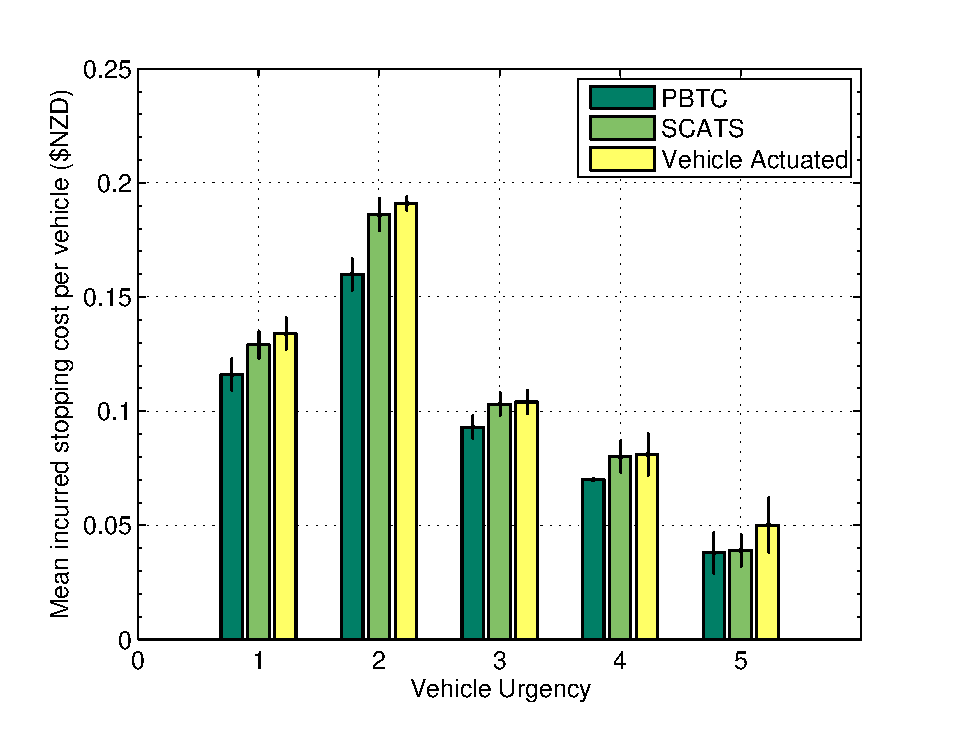
\includegraphics[scale=0.5]{vivian_victoria_approaches_stopping_cost.eps}
  \caption{Vivian-Victoria}
  \label{mean_stopping_cost:sub1}
\end{subfigure}%
\begin{subfigure}{.5\textwidth}
  \centering
  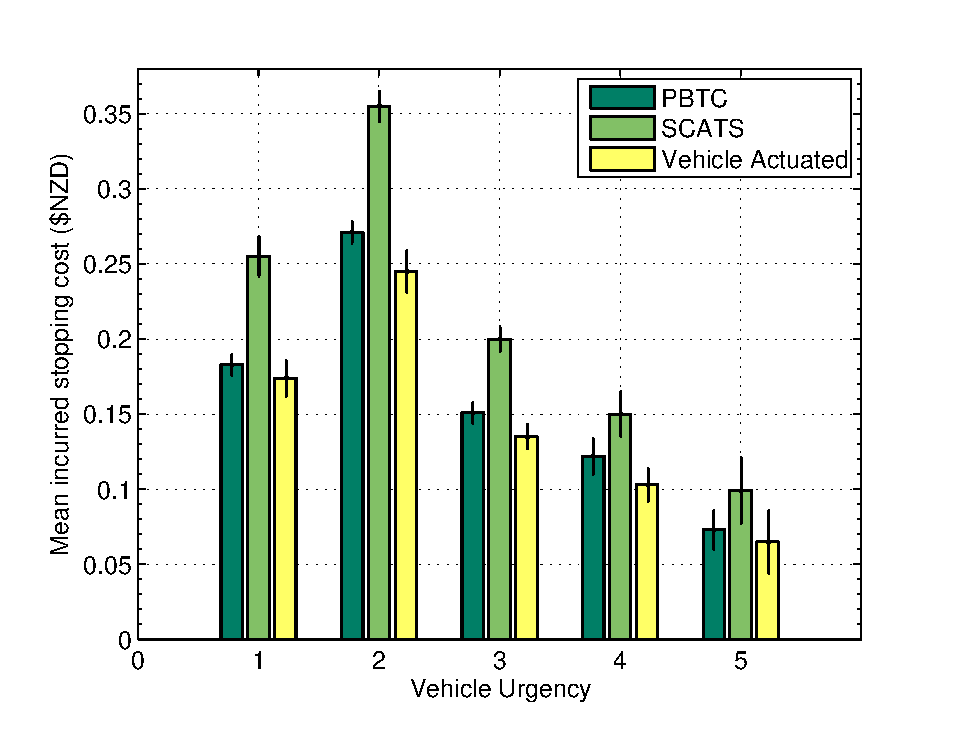
\includegraphics[scale=0.5]{courtenay_tory_approaches_stopping_cost.eps}
  \caption{Courtenay-Tory}
  \label{mean_stopping_cost:sub2}
\end{subfigure}

\vspace{1cm}

\begin{subfigure}{.5\textwidth}
  \centering
  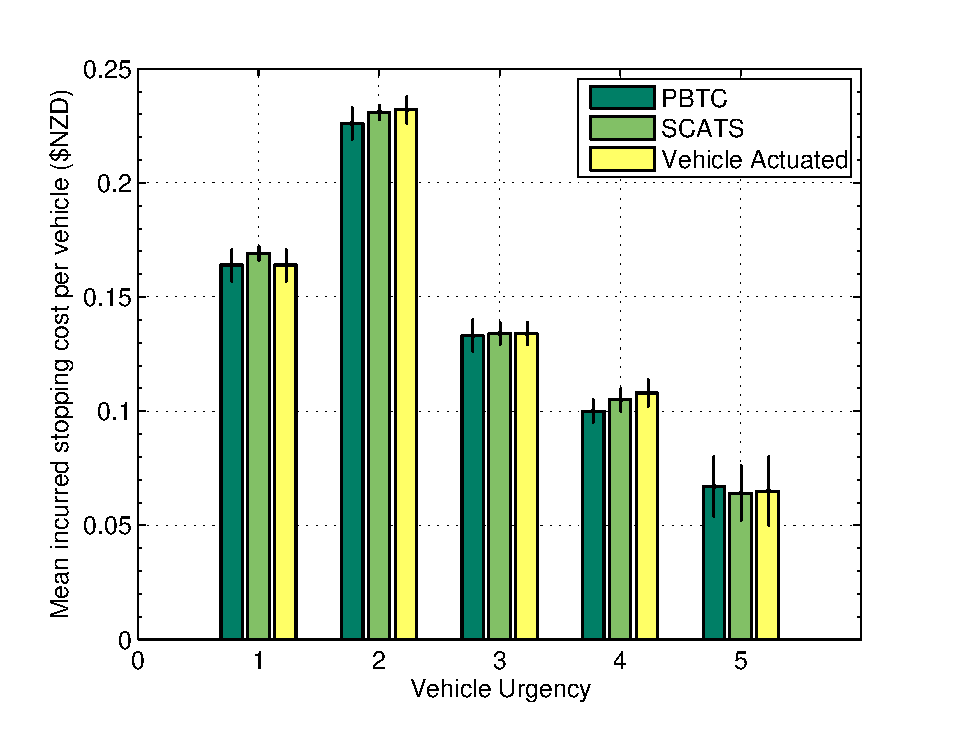
\includegraphics[scale=0.5]{karo_victoria_approaches_stopping_cost.eps}
  \caption{Karo-Victoria}
  \label{mean_stopping_cost:sub3}
\end{subfigure}%
\caption{ A bar chart of the mean incurred stopping cost of an individual vehicle, in New Zealand Dollars, for each of the three simulated intersections. The PBTC system consistently achieves lower mean stopping costs for vehicles in the simulation, although the performance of the SCATS and Vehicle Actuated systems is much more comparable than performance with respect to mean delay cost.   }
\label{eval:mean_stopping_cost}
\end{figure}

There is a consistent trend of decreasing stopping cost as urgency increases over all of the control strategies for the three evaluation intersections. This trend is accordant with the distribution of vehicle urgencies shown in Table ~\ref{urgencydistribution}, as the probability of an heavy vehicle with a large cost of stopping (e.g. bus or commercial truck) having a higher urgency value is comparatively low, and not possible in the case of urgency 5. The highest recorded mean stopping costs are observed for urgency 2 vehicles, which conforms to this conclusion. %why?

\begin{figure}
\centering
\begin{subfigure}{.5\textwidth}
  \centering
  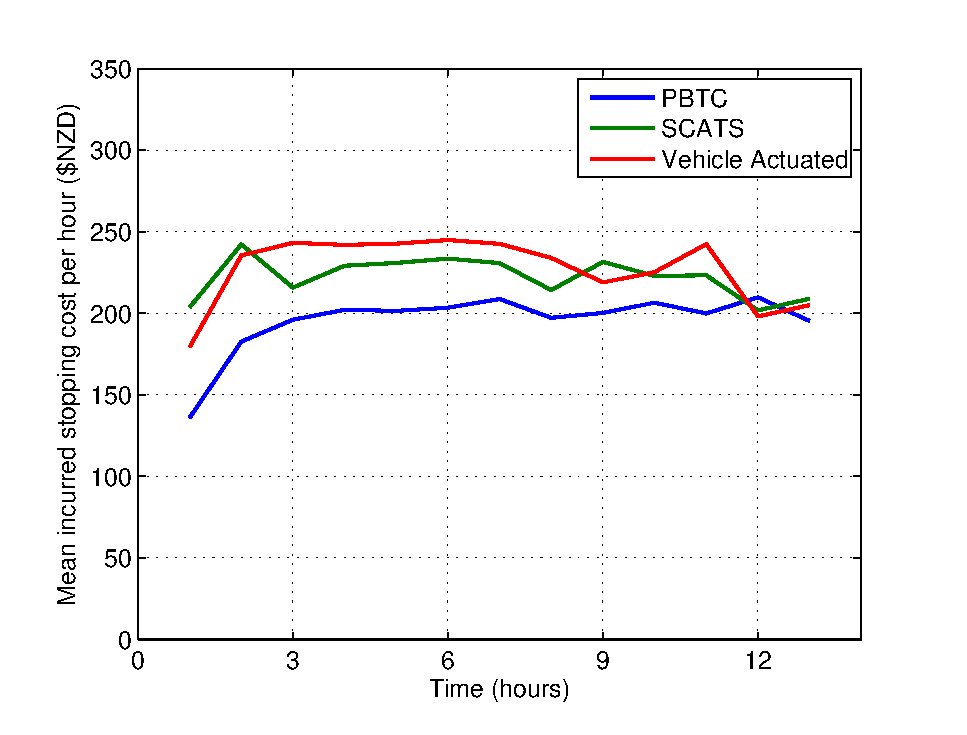
\includegraphics[scale=0.5]{vivian_victoria_stopping_cost_time.eps}
  \caption{Vivian-Victoria}
  \label{stopping_cost_time:sub1}
\end{subfigure}%
\begin{subfigure}{.5\textwidth}
  \centering
  \includegraphics[scale=0.5]{courtenay_tory_stopping_cost_time.eps}
  \caption{Courtenay-Tory}
  \label{stopping_cost_time:sub2}
\end{subfigure}

\vspace{1cm}

\begin{subfigure}{.5\textwidth}
  \centering
  \includegraphics[scale=0.5]{karo_victoria_stopping_cost_time.eps}
  \caption{Karo-Victoria}
  \label{stopping_cost_time:sub3}
\end{subfigure}%
\caption{ A plot of the mean incurred stopping cost per hour for each of the PBTC, SCATS, and Vehicle Actuated control strategies as applied to each of the three evaluation intersection configurations. Each plot line displays an indication of the trend in stopping cost over the period of a day.  }
\label{eval:stopping_cost_time }
\end{figure}

Figure ~\ref{eval:mean_stopping_cost} also shows that the PBTC control strategy performs well with regards to reducing the mean stopping cost at all three evaluation intersections, outperforming both the SCATS and Vehicle Actuated systems over a majority of the vehicle urgency values, but by only a small margin in most cases. It is important to note the cost of stopping is closely related to the speed of vehicles flowing through the system and the cost of stopping individual vehicles travelling slowly in a queue is appreciably lower than stopping freely flowing vehicles traveling at the speed limit of the area, due to the lower instantaneous velocity at the point of stopping. As a result, an inverse relationship exists between delay cost and incurred stopping cost with respect to vehicle speed. This result can be used to explain the similar performance of the SCATS and Vehicle Actuated control strategies when compared to the performance of the PBTC system. As the mean delay time per vehicle achieved by the SCATS and Vehicle Actuated strategies is greater, the length of vehicle queues is higher as more vehicles are delayed at the intersection, and as a result the cost of stopping a slowly moving queue is far less than stopping the same vehicles at higher speeds.

The relationship between time of day and mean stopping cost recorded per hour is shown in Figure ~\ref{eval:stopping_cost_time}. The performance of the three control strategies is relatively similar over each of the three evaluation intersections, although the mean stopping cost per hour recorded by the SCATS system appears to be consistently higher over the duration of the evaluation period. The mean stopping cost per hour measured for each of the PBTC and Vehicle Actuated control strategies is similar and varies between the three evaluation intersections. Given that the mean delay time over these periods is significantly lower for the PBTC system, the lower mean stopping cost is a benefit of the strategy itself, rather than long delay/slower traffic as is the case for the SCATS and Vehicle Actuated systems.
% do we need to back this up with queue stats?

\section{Overall Incurred Costs}

The overall incurred cost of operation over the evaluation period is an important metric as the primary goal of the PBTC system is to reduce the overall operation costs by including consideration of individual vehicle costs in traffic control  decisions. Figure ~\ref{eval:total_cost} shows the mean and standard deviation of the total overall costs measured for 10 simulation runs on each of the simulated intersections. The same data is also displayed in Table ~ref{eval:total_costs_table}.

The PBTC control strategy achieves the lowest mean total cost over all three simulated intersections, with between 13.7\% and 32.5\% reduction in overall costs compared to the SCATS control strategy, and 13.9\% to 19.0\% when compared to the Vehicle Actuated strategy. This result is supported by the results of the previous sections, where the PBTC control system is able to achieve the lowest delay times, and delay costs and incurred stopping costs, for all of the simulated intersections. 

These results also show that the Vehicle Actuated control strategy outperforms SCATS with respect to the mean total cost for the evaluation period for the Courtenay-Tory and Karo-Victoria intersections. The results of sections ~\ref{sec:incurred_delay_cost}~ and \ref{sec:incurred_stopping_cost} show that SCATS performs significantly worse with respect to delay cost at the Karo-Victoria intersection and stopping cost at the Courtney-Tory intersection, respectively.

For the Courtenay-Tory intersection, mean stopping cost per vehicle is a more significant factor that accounts for a larger proportion of the overall costs incurred during intersection operation. As previously described, the relatively poor performance of the Vehicle Actuated strategy with respect to delay time creates long, slow-moving vehicle queues; where stopping the queue does not incur significant stopping cost for each individual vehicle and as a result the overall cost is observed to be lower than that of SCATS. Although this result appears positive for the Vehicle Actuated strategy, in practice the long delay times are undesirable and increase the potential for queues to limit the throughput of the infrastructure to the point where the network reaches a ``gridlock'' preventing queues from clearing. 

\begin{figure}
\centering
\begin{subfigure}{.5\textwidth}
  \centering
  \includegraphics[scale=0.5]{vivian_victoria_approaches_total_cost.eps}
  \caption{Vivian-Victoria}
  \label{total_cost:sub1}
\end{subfigure}%
\begin{subfigure}{.5\textwidth}
  \centering
  \includegraphics[scale=0.5]{courtenay_tory_approaches_total_cost.eps}
  \caption{Courtenay-Tory}
  \label{total_cost:sub2}
\end{subfigure}

\vspace{1cm}

\begin{subfigure}{.5\textwidth}
  \centering
  \includegraphics[scale=0.5]{karo_victoria_approaches_total_cost.eps}
  \caption{Karo-Victoria}
  \label{total_cost:sub3}
\end{subfigure}%
\caption{The intersection of Vivian Street and Victoria Street in Te Aro, Wellington City, as viewed in the SCATS management application in use by Wellington City Council. }
\label{eval:total_cost}
\end{figure}

The results presented in this experimental evaluation support the notion of a cost tradeoff between stopping a currently flowing traffic approach and delaying all other competing approaches, the design basis of the PBTC system. To analyse how each of the strategies evaluated balances these cost values, Figure ~\ref{eval:cycle_durations} shows a plot of the mean cycle duration for each of the three control strategies over the period of each simulation. Of each of the three systems, the PBTC control strategy typically operates the longest cycle durations.

The chart ~\ref{cycle_durations:sub1} shows a clear example of the different phase durations operated by each of the control strategies. Between 8 and 12 hours, the PBTC control strategy fluctuates sharply between 130 and 160 seconds. As the PBTC control algorithm adapts to real-time traffic demand based on vehicles present and within range, more pronounced peaks of extended duration are expected. In contrast, the Vehicle Actuated control strategy has very little cycle duration variance and the recorded cycle duration does not exceed 110 seconds for the same period, due to the fixed phase durations operated by this strategy. The same period also shows evidence of incremental adaptation of the SCATS control algorithm, as the mean cycle duration increases by 40 seconds over a 2 hour period. 

Small periods of long cycle durations for each of the systems are observed during times of low traffic demand, where a phase is extended beyond its typical duration because no competing phases are demanded. This is most obvious on the Courtney-Tory and Karo-Victoria intersections, where the trend of mean cycle duration for SCATS fluctuates over the middle of the day. Referring to the trend in vehicle arrivals shown in \ref{eval:vehicle_arrivals_time} it is shown that at least one of the approaches to each intersection recorded relatively low traffic volumes at this time, explaining the lack of competing demand and extended phase durations.

The mean cycle durations operated by SCATS for the Courtenay-Tory intersection explains the observed period of significantly high mean delay costs for individual vehicles shown in ~\ref{delay_cost_time:sub2}. Figure ~\ref{cycle_durations:sub2} shows that over this period the mean cycle durations operated by SCATS were very low when compared to the PBTC and Vehicle Actuated strategies. The lower cycle duration over this period results in a larger number of phase changes and greater proportion of lost effective green time on both approaches, leading to longer queues and the observed jump in mean delay cost incurred. 

\begin{table}[]
\begin{center}
\begin{tabular}{llrlrlr}
\toprule
 & \multicolumn{2}{c}{Vivian-Victoria} & \multicolumn{2}{c}{Courtenay-Tory} & \multicolumn{2}{c}{Karo-Victoria} \\
 \cmidrule(lr){2-3}
 \cmidrule(lr){4-5}
  \cmidrule(lr){6-7}
Strategy &  Total Cost & \Delta\% & Total Cost & \Delta\% & Total Cost & \Delta\% \\
\midrule
PBTC & 4336.15 (\pm 34.8) &  & 1696.96 (\pm 31.2) & & 4051.84 (\pm 50.9) & \\
SCATS & 4928.21 (\pm 38.9) & +13.7\% & 2294.13 (\pm 31.1) & +35.2\%  & 4859.15 (\pm 48.0) & +19.9\% \\ 
VA & 5161.13 (\pm 27.5) & +19.0\% & 1969.76 (\pm 18.1) & +16.1\% & 4615.98 (\pm 45.3) & +13.9\% \\
\bottomrule
\end{tabular}
\end{center}
\caption{ Mean total cost (NZD) of ten simulation runs, and percentage difference relative to the performance of the PBTC system for each of the three control strategies and intersection examples used in evaluation. Mean total cost error is the standard deviation of the mean total cost for ten simulation runs. The PBTC control system achieves between 13.7\% and 35.2\% reduction of the total costs of operation over the 13-hour evaluation period. }
	\label{eval:total_costs_table}
\end{table}

\begin{figure}
\centering
\begin{subfigure}{.5\textwidth}	
  \centering
  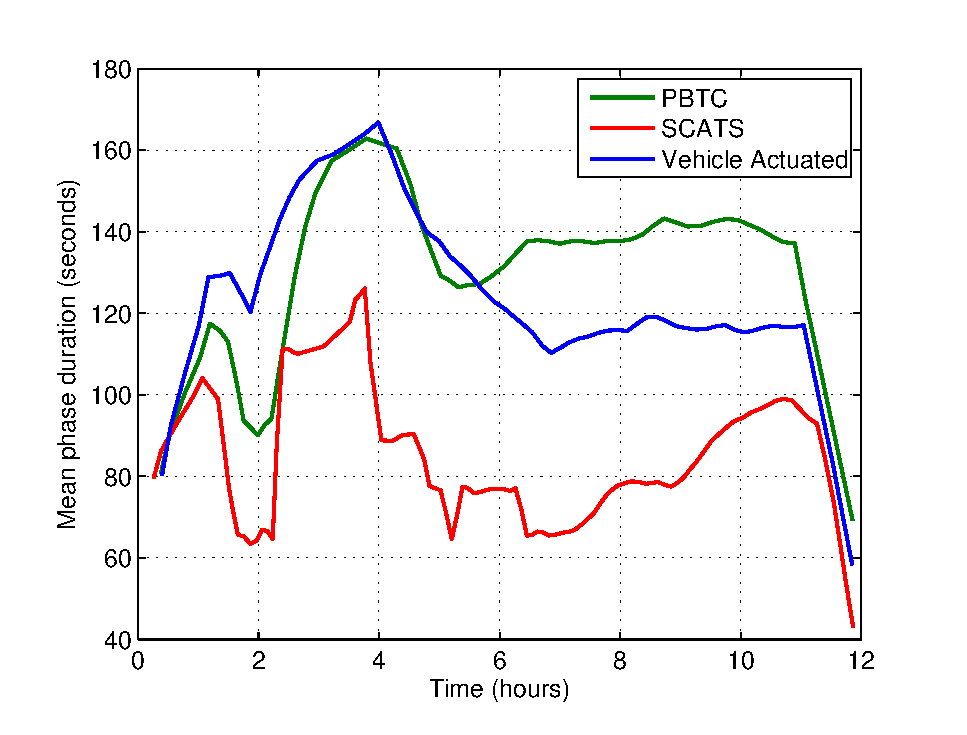
\includegraphics[scale=0.5]{vivian_victoria_cycle_durations.eps}
  \caption{Vivian-Victoria}
  \label{cycle_durations:sub1}
\end{subfigure}%
\begin{subfigure}{.5\textwidth}
  \centering
  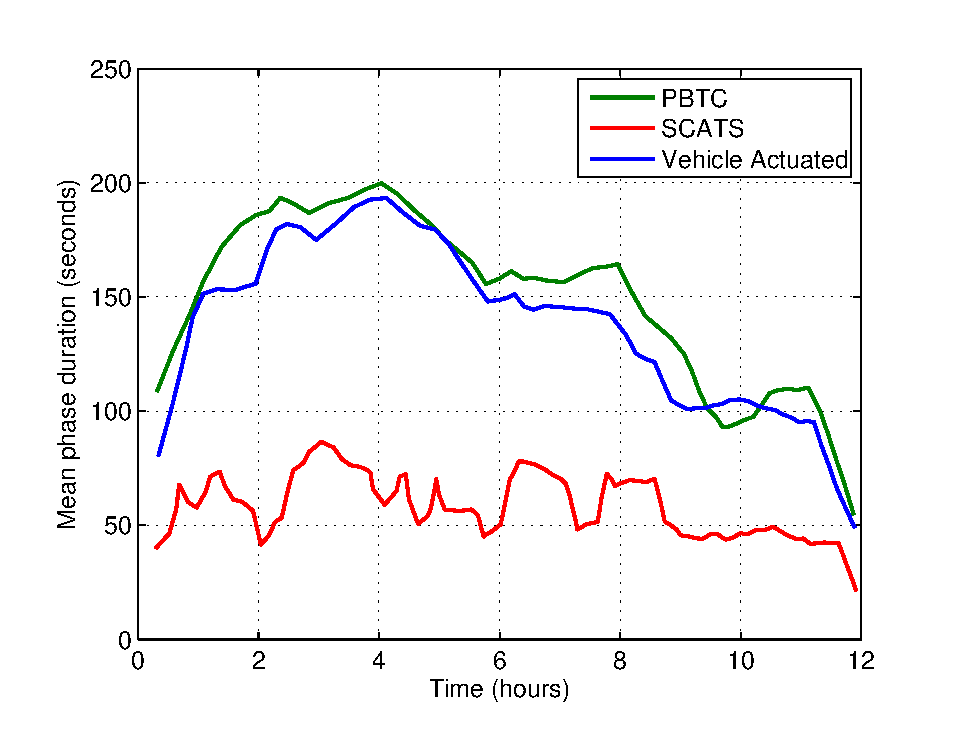
\includegraphics[scale=0.5]{courtenay_tory_cycle_durations.eps}
  \caption{Courtenay-Tory}
  \label{cycle_durations:sub2}
\end{subfigure}

\vspace{1cm}

\begin{subfigure}{.5\textwidth}
  \centering
  \includegraphics[scale=0.5]{karo_victoria_cycle_durations.eps}
  \caption{Karo-Victoria}
  \label{cycle_durations:sub3}
\end{subfigure}%
\caption{ A plot of the mean cycle duration in seconds for each of the PBTC, SCATS, and Vehicle Actuated control strategies over each of the simulated intersections. The cycle duration is calculated by adding the durations of each pair of phases in the system. The PBTC and Vehicle Actuated strategies are closely related as they both operate on the basis of real-time vehicle detections/communication broadcasts. Large peaks are observed whenever periods of low traffic volume cause a phase to be extended due to no competing demand.  }
\label{eval:cycle_durations}
\end{figure}

\section{Discussion}

The results presented in this chapter show the design of the PBTC control algorithm successfully reduces time spent delayed, costs incurred by delay, and costs incurred by stopping compared to the SCATS and Vehicle Actuated control strategies for all of the simulated intersections used in evaluation. In addition, the PBTC control system is able to prioritise vehicles based on their urgency, decreasing the delay time for vehicles with a higher relative urgency of travel.

\subsection{Validity}

A considerable effort has been made to ensure the validity and applicability of the results generated by this project. Design decisions related to the traffic priority model used to estimate journey costs; software design of PBTSim for simulation; and design and implementation of the PBTC control strategy, Vehicle Actuated control strategy, and SCATS representation; have been carefully considered to model realistic traffic scenarios. Threats to validity are based upon the assumptions made when designing estimate models, and representation of the traffic composition and SCATS behaviour during experimental evaluation.

\subsubsection{Priority Modeling for Cost Estimation}

The priority model designed during this project was required for the design and development of the PBTC system, and evaluation of the performance of the three control strategies tested during experimental evaluation. Cost of delay and cost of stopping are the primary components of this model. These costs are quantifiable and based on existing implicit costs incurred by motorists on real-world road networks. 

To calculate the cost of delay, a model has been designed based on the New Zealand Transport Agency recommended figure of \$26.20 New Zealand Dollars per vehicle hour, as opposed to an arbitrarily designed numerical value with no research as the basis of quantification. For the purposes of this project, this value is assumed to be correct for all vehicles on New Zealand roads. 

To calculate the cost of stopping a vehicle, a physics based fuel consumption model has been designed based on the kinetic energy required to accelerate a vehicle to a given speed, and the amount of speed effectively ``lost'' when a vehicle is forced to stop their journey at a controlled intersection. This model is limited by lack of consideration of different engine efficiencies, power to consumption ratios of different vehicle gears, and driver behaviours; all of which can improve or deteriorate the costs of fuel consumption involved in a forced stop. The separation of simulation vehicles into fixed property light or heavy classes is a significant simplification which doesn't accurately model realistic traffic composition on New Zealand roads. It is expected that more sophisticated modeling may influence the cost values produced by experimentation, but consistently, so the performance of each of the control strategies will not be affected.

\subsubsection{SCATS Log Data}

 This project relies on the data contained in log files produced by the SCATS system operating in Wellington City and provided by the Wellington City Council for simulation of traffic volume and experimental evaluation of the performance of the SCATS control strategy with regards to delay and stopping cost incurred with prioritised traffic.
 
The use of logged SCATS data introduces threats to the validity of experimental results. The SCATS log files are poorly labeled and can contain up to four detectors per approach. It is often unclear exactly which detectors are recording logged data without specific knowledge of the configuration on a per intersection basis. The software package designed to parse SCATS logs within PBTSim assumed that all approach data for each labelled approach identified of interest was relevant, with the exception of the Courtenay-Tory intersection where this behaviour was overridden to exclude data that was known to relate to the omitted turning lanes of both streets. The accuracy of detector data in the SCATS log file for the Karo-Victoria intersection should be doubted, as the SCATS representation consistently performed worse on this intersection compared to Vivian-Victoria and Courtenay-Tory across all evaluation metrics, and the measured flow rate at Victoria Street was significantly less than expected.

The SCATS log data is also used to set the phase times for the SCATS system during simulation. While these phase durations can be expected to be correct, because vehicle arrivals are simulated using the Poisson process there is no certainty that the vehicles present at any instantaneous moment of simulation are reliably reflective of the real-world demand that the SCATS system responded to. More robust evaluation is suggested as an area of future work for this project.



\chapter{Discussion}

The PBTC system achieves reduced delay times, without significant increases to the cost of stopping for all vehicles approaching an intersection, while prioritising traffic based on urgency and reducing the total trip time for vehicles whose transit is deemed to be urgent. 

%%%%%%%%%%%%%%%%%%%%%%%%%%%%%%%%%%%%%%%%%%%%%%%%%%%%%%%
\backmatter
%%%%%%%%%%%%%%%%%%%%%%%%%%%%%%%%%%%%%%%%%%%%%%%%%%%%%%%

%\bibliographystyle{ieeetr}
\bibliographystyle{acm}

\bibliography{sample}

\begin{appendices}

\chapter{Terminology}
\label{appendix:terminology}

Traffic control engineering involves specific terminology to refer to different signal controls, timing plans, and controller types. This section offers a brief introduction of traffic signal control and terminology.

Modern intersections with traffic signals are controlled by a roadside \emph{signal controller}. An intersection consists of a number of \emph{approaches} which are distinct roads leading to a point of intersection. Controllers switch power to signal lanterns and determine the sequence of display for each set of lights, operating under the safety requirement that no two conflicting approaches receive green signals simultaneously. A typical controller operates lights in sequences called \emph{phases}, which are dynamic length allocations of green light time to a set of non-conflicting flows at an intersection. \cite{papa2003review}. Typically, modern controllers include the following fixed or dynamic time allocations within a phase:

\begin{itemize}
\item \emph{late start time}, a fixed length of time a green light may be delayed for safety of other movements (e.g. pedestrian protection)
\item \emph{minimum green time}, a fixed length of time that a phase must operate before changing
\item \emph{intergreen time}, a fixed length of time required to operate amber and red signals at the end of a phase, typically at least 6 seconds. 
\item \emph{extension green time}, a dynamic length of time allocated to a phase determined after all required fixed times have been deducted from the total phase tie. 
\item \emph{maximum green time}, if the addition of the previous four time allocations exceeds the fixed maximum green time the phase is forced to change. 
\end{itemize}

A \emph{cycle} (or \emph{plan}) is an ordered sequence of one or more phases which is repeated by a controller. A fixed cycle traffic controller runs each phase for a fixed length of time within a static cycle. An actuated traffic controller can respond to sensor inputs from lane road loops and skip phases that are not in demand. Adaptive traffic controllers differ in implementation but typically can extend or shorten the length of a phase if a queue is completely cleared midway through a phase. The length of a cycle of an adaptive controller can be adapted to demand, typically running for a shorter length of time during quiet traffic and increasing in length to reduce queuing and satisfy high demand peaks \cite{scatstraining}.

An intersection has a given \emph{capacity}, defined as the maximum sustainable flow rate at which vehicles or pedestrians can travel through the intersection in a given time period. Capacity is dependant on the geometric layout of an intersection (e.g. width of road, number of lanes), driving and surface conditions, and traffic conditions. The \emph{degree of saturation} of an intersection is a ratio of arrival flow rate with respect to capacity of each approach for a given period. Arrival flow rate, also called \emph{demand flow}, refers to the number of vehicles or pedestrians arriving during a given period, measured from the back of a queue \cite{sidraglossary}. A section of road is said to be saturated if the traffic flow is equivalent to the capacity of the road at a given speed, such that any increase in flow will have a negative impact on the flow through the system. Any section of road where demanded traffic flow exceeds capacity is said to be \emph{congested} \cite{wallis2013costs}.

\chapter{Inter-Vehicle Communication}
\label{appendix:inter-vehicle-comms}

The ubiquity of mobile communication devices and modern wireless capabilities have offered new possibilities for inter-vehicle communication within road networks. Previous research suggests that short-range wireless communication devices installed in road vehicles can be used to form mobile ad-hoc networks between near proximity clusters of traffic \cite{adaptive2007grad,nadeem2004trafficview,yang2004vehicle}. Dedicated short-range communication (DSRC) is a standard for vehicle-to-vehicle and vehicle-to-infrastructure communication, currently under active development in the United States\cite{dsrc2011}.

Car-to-car communication and car-to-controller communication has been researched as a replacement for loop detection used by adaptive traffic controllers \cite{adaptive2007grad}. In this implementation, vehicles periodically transmit information about themselves and other nearby vehicles to a traffic controller using one-hop broadcasts. A traffic signal controller maintains a record of each known vehicle within range and optimises cycle length and phase timings based for the succeeding phase based on real-time information from each approach. Experimentation results suggest that adaptive traffic control using a simple traffic actuated method out-performs a predetermined phase controller by a significant factor when total intersection delay is the primary measure of effectiveness at an intersection. While these results are promising, the work is limited in scope by the use of a predetermined phase time controller as a baseline for experimentation. The increase in performance measured by the authors does not take into account the advantages of existing traffic actuated or adaptive controller schemes over an isolated, fixed-cycle controller which are likely to be significant. 

Wireless communication between vehicles and signal controllers can provide more information at an earlier stage of approach than loop detectors, including characteristics of a vehicle (number of passengers, size, weight, type of activity), speed of approach and current position. Research in this field has explored the use of vehicle-to-vehicle communication for early warning safety systems, collision avoidance, and as a means of informing vehicle passengers about road network conditions; suggesting widespread benefits for use of the technology beyond traffic modeling at controlled intersections \cite{nadeem2004trafficview,yang2004vehicle}. 

\chapter{PBTC Control Algorithm}
\label{appendix:pbtc_algorithm}

Pseudocode for the PBTC control algorithm described in \ref{sec:PBTCDesign} is given below. The algorithm determines whether a phase change sequence is required and if so, determines the length of time the current phase duration should be extended based on estimates of the delay and stopping cost incurred by vehicles up to $K$ seconds into the future.

\begin{algorithm}[H]
 \SetAlgoLined
 \KwData{
 	$Approaches$: set of approaches, $K$: lookahead window size
 }
 \KwResult{ time in seconds before phase change should be executed or -1 for no change }
 \Begin{
  set $totalStoppingCost$ = 0 \; \\
  set $totalDelayCost$ = 0 \; \\
  \For{approach in $Approaches$}{
  	\If{approach signal is red} {
		add cost of delay for all vehicles queued on approach to $totalDelayCost$ \;
	} 
	\Else{
		add cost of stopping and cost of minimum delay for all vehicles on approach to $totalStoppingCost$ \;
	}
  }
  \If {$stoppingCost < delayCost$} {
  	set $lookaheadTable$ = [] \;
	\For{$i := 0$ to $K$} {
		$lookaheadTable$[$i$] = cost of delay for all stopped approaches over $i$ + cost of stopping for all vehicles that cannot clear the intersection within $i$ seconds \;
	}

  set $extendedGreenTime$ = index of min($lookaheadTable$) \; \\
  return $extendedGreenTime$ \;
}
return -1 \;	 \tcc*[r]{no change scheduled}
 }
 \caption{PBTC phase scheduling algorithm}
\end{algorithm}

\chapter{SCATS Data File Format}
\label{appendix:scats_data_file}

This section contains an excerpt from a data file generated by the SCATS TrafficReporter application, and provided to this project by the Wellington City Council for research purposes. The data shown represents three cycles of SCATS operation at the intersection of Victoria Street and Vivian Street in Central Wellington, between 6:00AM and 6:02AM on the 20th June, 2013. An brief explanation of the format of relevant data is given below.

\begin{verbatim}
Thursday 20-June-2013 06:00 SS   3   PL 5.3  PVa3.3 CT   65 +0 RL 65, SA 10  DS 44
 Int   SA/LK    PH  PT!  DS  VO  VK!  DS  VO  VK!  DS  VO  VK!  DS  VO  VK! ADS
  520 S  10  '   A  36!  64  10  10!  57   9  10!   -       -!   -       -!   44
  520 S  11 ^    2  26!  17   2   2!   0   0   0!   -       -!   -       -!   19
  530 S  12 *'   A  35!  57   9   8!  41   7   6!   -       -!   -       -!   35
  530 S  13      B  24!  30   4   3!  16   2   2!  15   2   2!   -       -!   14
  520 S 273 ^    B  26!  17   2   2!   -       -!   -       -!   -       -!   23
A=<65>  B=35
Thursday 20-June-2013 06:01 SS   3   PL 5.3  PVa2.3 CT   65 +0 RL 65, SA 10  DS 54
 Int   SA/LK    PH  PT!  DS  VO  VK!  DS  VO  VK!  DS  VO  VK!  DS  VO  VK! ADS
  520 S  10  '   A  41!  43   8   7!  55  11  11!   -       -!   -       -!   54
  520 S  11 ^    2  25!  14   2   2!  56   4   6!   -       -!   -       -!   36
  530 S  12 *'   A  67!  26   8   7!  36  11  10!   -       -!   -       -!   40
  530 S  13      B   0!   0   0   0!   0   0   0!   0   0   0!   -       -!   10
  520 S 273 ^    B  25!   0   0   0!   -       -!   -       -!   -       -!   13
A=<64>  B=36
Thursday 20-June-2013 06:02 SS   3   PL 5.3  PV 0.3 CT   65 +0 RL 65, SA 10  DS 44
 Int   SA/LK    PH  PT!  DS  VO  VK!  DS  VO  VK!  DS  VO  VK!  DS  VO  VK! ADS
  520 S  10  '   A  65!  27   9   7!  21   8   6!   -       -!   -       -!   44
  520 S  11 ^    2   0!   0   0   0!   0   0   0!   -       -!   -       -!   22
  530 S  12 *'   A  41!  12   3   2!  34   7   6!   -       -!   -       -!   40
  530 S  13      B  23!  11   2   1!   0   0   0!   0   0   0!   -       -!   12
  520 S 273 ^    B   0!   0   0   0!   -       -!   -       -!   -       -!    4
A=<64>  B=36
\end{verbatim}

\begin{itemize}
\item \textbf{Int} Intersection, the unique identifier of the intersection each data line corresponds to. Some log files can include data from nearby intersections to help traffic engineers report on an entire subsystem. The snippet above shows data for intersections 520 and 530.
\item \textbf{SA/LK} Strategic Approach/Link, the identifier to describe an approaching road, unique within an intersection.
\item \textbf{PH} Phase, the alphabetical character identifier used to name the phase that was operated. Typically the letters A-F are used to describe each phase. 
\item \textbf{PT!} Phase time, the duration in seconds of the phase that was operated.
\item \textbf{DS} Degree of Saturation, the degree of saturation measured for traffic flow during the cycle.
\item \textbf{VO} Vehicle actuations, the number of vehicles that were counted by stop-line detectors during the cycle.
\end{itemize}

\chapter{Evaluation Intersections}
\label{appendix:scats_intersections}

Three intersections within the Wellington City central road network were selected as the basis for evaluation of this project. Figure \ref{intersectionmap} shows a map of Wellington City, marked with the location of the three intersections considered, Vivian Street and Victoria Street, Courtenay Place and Tory Street, and Karo Drive and Victoria Street. The intersections were selected based on the availability of logged data from the Wellington City Council, capability of the PBTSim simulator to model the intersections appropriately, and variations in traffic volume to investigate the performance of the PBTC control algorithm in multiple realistic traffic scenarios. The map shown was generated using Google Maps \cite{google-maps}.

\begin{figure}[]
\centering
	\includegraphics[scale=0.5]{intersection-map.pdf}
	\caption[A map of Wellington City showing intersections used for evaluation]{ A map of Wellington City showing the intersections of Vivian Street and Victoria Street, Courtenay Place and Tory Street, and Karo Drive and Victoria Street marked. }
\label{intersectionmap}
\end{figure}


\section{SCATS Representations} 

Figure \ref{scats_intersections} shows the three evaluation intersections used during evaluation of the PBTC system as represented in the SCATS system used by Wellington City Council. Screenshots were provided by Wellington City Council traffic engineers. The SCATS phase configuration for each intersection is shown to the left of each figure. Note that in the case of Courtenay-Tory, phases A, B, C, E, E1, and E2 are considered as a single phase in the SCATS log files and PBTSim configuration.


\begin{figure}[]
\centering
\begin{subfigure}{.5\textwidth}
  \centering
  \includegraphics[scale=0.35]{scats-vivian-victoria.png}
  \caption{Vivian Street-Victoria Street}
  \label{fig:sub1}
\end{subfigure}%
\begin{subfigure}{.5\textwidth}
  \centering
  \includegraphics[scale=0.35]{scats-courtenay-tory.png}
  \caption{Courtenay Place-Tory Street}
  \label{fig:sub2}
\end{subfigure}

\vspace{1cm}

\begin{subfigure}{.5\textwidth}
  \centering
  \includegraphics[scale=0.35]{scats-karo-victoria.png}
  \caption{Karo-Victoria}
  \label{fig:sub1}
\end{subfigure}%
\caption{ Screenshots of the Vivian-Victoria, Courtenay-Tory, and Karo-Victoria intersections as represented in the SCATS system. }
\label{scats_intersections}
\end{figure}

\section{PBTSim Representations}

Figure \ref{pbtsim_intersections} shows the visual representation of the three evaluation intersections within the PBTSim graphical user interface. All lanes catering for turning traffic have been omitted from each intersection and are not considered by this project. 

\begin{figure}[]
\centering
\begin{subfigure}{.5\textwidth}
  \centering
  \includegraphics[scale=0.35]{pbtsim-vivian-victoria.png}
  \caption{Vivian-Victoria}
  \label{fig:sub1}
\end{subfigure}%
\begin{subfigure}{.5\textwidth}
  \centering
  \includegraphics[scale=0.35]{pbtsim-courtenay-tory.png}
  \caption{Courtenay-Tory}
  \label{fig:sub2}
\end{subfigure}

\vspace{1cm}

\begin{subfigure}{.5\textwidth}
  \centering
  \includegraphics[scale=0.35]{pbtsim-karo-victoria.png}
  \caption{Karo-Victoria}
  \label{fig:sub1}
\end{subfigure}%
\caption[Screenshows of the Vivian-Victoria, Courtenay-Tory, and Karo-Victoria intersections as represented in the PBTSim simulator.]{ Intersections of Vivian-Victoria, Courtenay-Tory, and Karo-Victoria as represented in the PBTSim simulator.  }
\label{pbtsim_intersections}
\end{figure}

\end{appendices}


\end{document}
